\documentclass{article}


% if you need to pass options to natbib, use, e.g.:
%     \PassOptionsToPackage{numbers, compress}{natbib}
% before loading neurips_2022
\PassOptionsToPackage{numbers, compress}{natbib}

% ready for submission
\usepackage[final]{neurips_2023}


% to compile a preprint version, e.g., for submission to arXiv, add add the
%[preprint] option:
%\usepackage[preprint]{neurips_2022}


% to compile a camera-ready version, add the [final] option, e.g.:
%     \usepackage[final]{neurips_2022}


% to avoid loading the natbib package, add option nonatbib:
%    \usepackage[nonatbib]{neurips_2022}


\usepackage[utf8]{inputenc} % allow utf-8 input
\usepackage[T1]{fontenc}    % use 8-bit T1 fonts
\usepackage{hyperref}       % hyperlinks
\usepackage{graphicx}
\usepackage{caption}
\usepackage{subcaption}% hyperlinks
\usepackage{url}            % simple URL typesetting
\usepackage{booktabs}       % professional-quality tables
\usepackage{amsfonts}       % blackboard math symbols
\usepackage{nicefrac}       % compact symbols for 1/2, etc.
\usepackage{microtype}      % microtypography
%\usepackage{xcolor}         % colors
\usepackage{bbold}
\usepackage{amsmath}
\usepackage{amsfonts}
\usepackage{amssymb}
\usepackage{bm}

%\usepackage{unicode-math}
\usepackage{bbm}
\usepackage[normalem]{ulem}
%\usepackage{sout}
\usepackage{multirow}

\usepackage{cleveref}
\usepackage[table,xcdraw]{xcolor}
\newcommand{\Deellip}{
    \textit{DEEL.LIP}\footnote{\url{https://github.com/deel-ai/deel-lip} distributed under MIT License (MIT)}
}

\usepackage{graphicx}
%\usepackage{xcolor}

\newcommand{\W}{\mathcal{W}}
\newcommand{\x}{\bm{x}}
\newcommand{\X}{X}
\newcommand{\Y}{Y}
\newcommand{\y}{y}
\newcommand{\z}{\bm{z}}
\newcommand{\f}{\bm{f}}
\newcommand{\tr}{\bm{\gamma}}

\newcommand{\inp}{\mathcal{X}}
\newcommand{\boundary}{\partial \inp}

% probability distributions
%\newcommand{\dpos}{\mathcal{P}}
%\newcommand{\dneg}{\mathcal{Q}}
\newcommand{\dpos}{\mu}
\newcommand{\dneg}{\nu}
\newcommand{\dx}{P_{\x}}
\newcommand{\dy}{P_{\y}}
\newcommand{\djoint}{P}

\DeclareMathOperator*{\argmax}{arg\,max}
\DeclareMathOperator*{\argmin}{arg\,min}
\DeclareMathOperator*{\sign}{sign}

\newcommand{\commentgreen}[1]{
    \textcolor{green}{ #1 }
}
\newcommand{\commentblue}[1]{
    \textcolor{blue}{Mathieu : #1 }
}

\definecolor{greenish}{RGB}{55, 157, 143}
\newcommand{\fel}[1]{{\color{greenish}[fel]: #1}}
\newcommand{\mathieu}[1]{{\color{blue}[Mathieu]: #1}}
\newcommand{\losshkr}{$\mathcal{L}^{hKR}_{\lambda,m}$}
\newcommand{\lossreg}{$\mathcal{L}^{hKR}_{\lambda,\alpha}$}

\newcommand{\onlyonelip}{1-Lipschitz}
\newcommand{\otnn}{OTNN}

\newtheorem{theorem}{Theorem}
\newtheorem{proposition}{Proposition}
\newtheorem{corollary}{Corollary}

\newcommand{\BlackBox}{\rule{1.5ex}{1.5ex}}  % end of proof
\newenvironment{proof}{\par\noindent{\bf Proof\ }}{\hfill\BlackBox\\[2mm]}

%\newcommand{\fel}[1]{{\color{purple}[fel]: #1}} 
\newcommand{\louis}[1]{\textcolor{green}{#1}}


\newcommand{\AddAnnex}{0}

%\title{Optimal transport, robustness and explainability for classification}
\title{On the explainable properties of 1-Lipschitz Neural Networks: An Optimal Transport Perspective}
%\title{An Optimal Transport Perspective on the Explainable Properties of 1-Lipschitz Networks}
%\title{On the explainable properties of 1-Lipschitz Neural Networks: An Optimal Transport Perspective}


% The \author macro works with any number of authors. There are two commands
% used to separate the names and addresses of multiple authors: \And and \AND.
%
% Using \And between authors leaves it to LaTeX to determine where to break the
% lines. Using \AND forces a line break at that point. So, if LaTeX puts 3 of 4
% authors names on the first line, and the last on the second line, try using
% \AND instead of \And before the third author name.

\author{
Mathieu Serrurier$^1$ \And Franck Mamalet$^2$ \And Thomas Fel$^{3,4}$ \And Louis Béthune$^1$ \And Thibaut Boissin$^2$\\
\\
$^1$Université Paul-Sabatier, IRIT, Toulouse, France\\
$^2$Institut de Recherche Technologique Saint-Exupéry, Toulouse, France\\
$^3$Carney Institute for Brain Science,Brown University, USA \\
$^4$Innovation \& Research Division, SNCF, France
}

%\author{
%Mathieu Serrurier\\
%Université Paul-Sabatier, IRIT\\
%Toulouse, France
%\And Franck Mamalet\\
%IRT Saint-Exupéry\\
%Toulouse, France
%\And Thomas Fel\\
%Carney Institute for Brain Science, \\ Brown University, USA \\
%Brown University\\
%\And Louis Béthune\\
%Université Paul-Sabatier, IRIT\\
%Toulouse, France
%\And Thibaut Boissin, \\
%IRT Saint-Exupéry\\
%Toulouse, France
%}

%  Mathieu Serrurier. \\
%  IRIT\\
%  \texttt{mathieu.serrurier@irit.fr} \\
  % examples of more authors
%  \And%
%  .... \\
%  \\
%  \texttt{.@..fr} \\
  % Coauthor \\
  % Affiliation \\
  % Address \\
  % \texttt{email} \\
  % \AND
  % Coauthor \\
  % Affiliation \\
  % Address \\
  % \texttt{email} \\
  % \And
  % Coauthor \\
  % Affiliation \\
  % Address \\
  % \texttt{email} \\
  % \And
  % Coauthor \\
  % Affiliation \\
  % Address \\
  % \texttt{email} \\



\begin{document}


\maketitle


\begin{abstract}
%Since \commentgreen{for classical neural networks}, the gradients of input features form the basis of most adversarial attack algorithms, Saliency Maps, which represent these gradients, \commentgreen{are noisy and } typically do not offer significant insights for Explainable AI (XAI). 
%In this paper, we demonstrate that while learning a 1-Lipschitz neural network with the dual loss of an optimal transportation problem, the vanilla Saliency Map of these models exhibits desirable XAI properties. 
%Moreover, they also exhibit remarkably high alignment with human explanations on ImageNet.
%These modifications are encoded by the Saliency Map. 



Input gradients have a pivotal role in a variety of applications, including adversarial attack algorithms for evaluating model robustness, explainable AI techniques for generating Saliency Maps, and counterfactual explanations.
However, Saliency Maps generated by traditional neural networks are often noisy and provide limited insights. 
In this paper, we demonstrate that, on the contrary, the Saliency Maps of 1-Lipschitz neural networks, learned with the dual loss of an optimal transportation problem, exhibit desirable XAI properties:
They are highly concentrated on the essential parts of the image with low noise, significantly outperforming state-of-the-art explanation approaches across various models and metrics. 
We also prove that these maps align unprecedentedly well with human explanations on ImageNet.
To explain the particularly beneficial properties of the Saliency Map for such models, we prove this gradient encodes both the direction of the transportation plan and the direction towards the nearest adversarial attack. Following the gradient down to the decision boundary is no longer considered an adversarial attack, but rather a counterfactual explanation that explicitly transports the input from one class to another. 
Thus, Learning with such a loss jointly optimizes the classification objective and the alignment of the gradient, i.e. the Saliency Map, to the transportation plan direction.
These networks were previously known to be certifiably robust by design, and we demonstrate that they scale well for large problems and models, and are tailored for explainability using a fast and straightforward method.


%In this paper, we demonstrate that while learning a 1-Lipschitz neural network with the dual loss of an optimal transportation problem, the model's gradient serves as both the direction of the transportation plan and the direction to the nearest adversarial attack. Following the gradient to the decision boundary is no longer considered an adversarial attack, but rather a counterfactual explanation that explicitly transports the input from one class to another. We conducted extensive experiments on XAI metrics and found that the simple Saliency Map method, when applied to such networks, is either equivalent or superior to more complex XAI methods. Moreover, our method outperforms the state-of-the-art explanation approaches on all types of models, exhibiting remarkable higher alignment to human explanations on imagenet. Our proposed networks were previously known to be certifiably robust by design, and we prove that they are tailored for explainability. using a fast and straightforward method. \commentblue{Ajouter qu'on est le premier en 1-Lip sur de grand réseaux ?}

\end{abstract}


\section{Introduction}
\label{sec:introduction}
\iffalse
Counterfactual explanations in classification demonstrate why a decision was made for option A instead of option B. In symbolic models, this modification can be significant and indicate causality between feature values and class \cite{Lewis1973}. However, in high-dimensional spaces where causal models are not available, this modification is reduced to an adversarial attack~\cite{Madry2017}. Adversarial attacks require carefully chosen small modifications, such as imperceptible noise, to change the class of an example and deceive the network. As a result, this noise does not typically provide genuine counterfactual explanation since it is counterfactual with respect to the model but not to the class \cite{wachter2017counterfactual}. Thus, Saliency Maps \cite{SimonyanVZ13} -- gradient of output with respect to the input --, which are the basis for most adversarial attacks, are generally unsuitable for explaining model decisions. Therefore, several methods requiring more complex computations, such as SmoothGrad \cite{Smilkov2017}, Integrated Gradient \cite{Sundararajan2017}, or Grad-CAM \cite{Selvaraju_2019}, have been proposed to provide better explanations. Recently, the XAI community has investigated the link between explainability and robustness and proposed methods and metrics accordingly~\cite{hsieh2020evaluations, boopathy2020proper, lin2019explanations, ross2021learning}.
In~\cite{serrurier2021achieving}, authors propose to address the weakness with respect to adversarial attacks by training \onlyonelip~constrained neural networks with a loss that is the dual of an optimal transport optimization problem, called hKR and noted \losshkr. The resulting models have been shown to be robust with a certifiable margin. We refer to these networks as Optimal Transport Neural Networks (\otnn) hereafter.
\fi


The Lipschitz constant of a function expresses the extent to which the output may vary for a small shift in the input. As a composition of numerous functions, the Lipschitz constant of a neural network can be arbitrarily high, particularly when trained for a classification task \cite{bethunelip}. Adversarial attacks~\cite{Madry2017} exploit this weakness by selecting minor modifications, such as imperceptible noise, for a given example to change the predicted class and deceive the network. Consequently, Saliency Maps \cite{SimonyanVZ13} -- gradient of output with respect to the input --, serve as the basis for most adversarial attacks and often highlight noisy patterns that fool the model instead of meaningful modifications, rendering them generally unsuitable for explaining model decisions. Therefore, several methods requiring more complex computations, such as SmoothGrad \cite{Smilkov2017}, Integrated Gradient \cite{Sundararajan2017}, or Grad-CAM \cite{Selvaraju_2019}, have been proposed to provide smoother explanations. Recently, the XAI community has investigated the link between explainability and robustness and proposed methods and metrics accordingly~\cite{hsieh2020evaluations, boopathy2020proper, lin2019explanations, ross2021learning}.
%\commentgreen{Such  automatic metrics can still suffer from biases, and no clear evidence that they are correlated with human notion of explanations. \cite{fel2022aligning} suggests comparing the alignment between attribution methods and human feature importance using the ClickMe dataset~\cite{linsley2017visual}.}
However, the reliability of those automatic metrics can be compromised by artifacts introduced by the baselines ~\cite{hsieh2020evaluations,sturmfels2020visualizing,haug2021baselines,kindermans2019reliability,hase2021out}, and there is no conclusive evidence demonstrating their correlation with the human understanding of explanations. To address this, a study by \cite{fel2022aligning} suggests completing those metrics with the alignment between attribution methods and human feature importance using the ClickMe dataset~\cite{linsley2017visual}.
%\mathieu{To obtain a metric that better mirrors human interpretation of decisions, \cite{fel2022aligning} suggests comparing the alignment between attribution methods and human feature importance using the ClickMe dataset~\cite{linsley2017visual}.}

In~\cite{serrurier2021achieving}, authors propose to address the weakness with respect to adversarial attacks by training \onlyonelip~constrained neural networks with a loss that is the dual of an optimal transport optimization problem, called hKR  (Eq.~\ref{eq:reg_OT}). The resulting models have been shown to be robust with a certifiable margin. We refer to these networks as Optimal Transport Neural Networks (\otnn) hereafter.

In this paper, we demonstrate that OTNNs exhibit valuable explainability properties. Our experiments reveal that OTNN Saliency Maps significantly outperform various attribution methods for unconstrained networks across all tested state-of-the-art Explainable XAI metrics. This improvement is consistent across toy datasets, large image datasets, binary, and multiclass problems. Qualitatively, OTNN Saliency Maps concentrate on crucial image regions and generate less noise than maps of unconstrained networks, as illustrated in Figure \ref{fig:big_picture}. Figure \ref{fig:big_picture}.c presents the Saliency Maps of an OTNN based on ResNet50 alongside its unconstrained vanilla counterpart, both trained on ImageNet~\cite{imagenet_cvpr09}. In the unconstrained case, the Saliency Maps appear sparse and uninformative, with the most critical pixels often located outside the subject. Conversely, the OTNN Saliency Map is less noisy and highlights significant image features. This distinction is emphasized in Figure \ref{fig:big_picture}.d), comparing the feature visualization of the two models. Feature visualization extracts the inverse prototypical image for a given class using gradient ascent \cite{olah2017feature,nguyen2016multifaceted}. The results for vanilla ResNet are noticeably noisy, making class identification difficult. In contrast, feature visualization with OTNN yields clearer results, displaying easily identifiable features and classes (e.g., goldfish, butterfly, and medusa). Furthermore, modifying the image following the gradient direction provides an interpretable method for altering the image to change its class. Pictures \ref{fig:big_picture}.a) and \ref{fig:big_picture}.b) display the original image, the gradient direction, and the transformation following the gradient direction (refer to Section 4 for details). We observe explicit structural changes in the images, transforming them into an example of another class in both multiclass (MNIST) and high-resolution multi-labels cases (e.g., smile/not smile and blond hair/not blond hair classification). Lastly, a large-scale human experiment demonstrates that these maps are remarkably aligned with human attribution on ImageNet (Fig. \ref{fig:human_alignement}).

%Fig. \ref{fig:mnist} illustrates, on an \otnn~learned on MNIST dataset, the transformation of an image of the class zero with respect to the gradient of another class's output (as done in a vanilla targeted attack). We observe that it explicitly changes the zero into the target number, and gradients provide understandable explanations of why it was not this number.

\begin{figure*}[ht]
  \centering
  %\fbox{
\includegraphics[width=0.95\linewidth]{img/mnist.png}}
  %\includegraphics[width=0.99\linewidth]{img/big_picture.jpg}
  \includegraphics[width=0.99\linewidth]{img/big_picturev_2.pdf}
\caption{
\textbf{Illustration of the beneficial properties of OTNN gradients.} Examples \textbf{a)} and \textbf{b)} show that the gradients naturally provide a direction that enables the generation of adversarial images - a theoretical justification based on optimal transport is provided in Section 3. By applying the gradient $\x' = \x  -t \nabla_{\x}  \f(\x)$ to the original image $\x$ (on the left), any digit from MNIST can be transformed into its counterfactual $\x'$ (e.g., turning a 0 into a 5). In \textbf{b)}, we illustrate that this approach can be applied to larger datasets, such as Celeb-A, by creating two counterfactual examples for the closed-mouth and blonde  classes. In \textbf{c)}, we compare the 
Saliency Map
%natural gradient 
of a classical model with those of OTNN gradients, which are more focused on relevant elements. Finally, in \textbf{d)}, we show that following the gradients of OTNN could generate convincing feature visualizations that ease the understanding of the model's features. 
}
\label{fig:big_picture}
\end{figure*}

%We provide a theoretical justification of the the well behavior of OTNN salency map. Starting from the fact that \otnn s~encode the dual formulation of the optimal transport problem, and we prove that the gradient of a given point $x$ is both (i) in the direction of the closest adversarial example on the decision boundary and (ii) in the direction of the image of $x$ according to the underlying transport plan. This implies that adversarial attacks for an \otnn~are equivalent to travels along the optimal transport path. As a result, the modification obtained is not only an adversarial attack but also a counterfactual explanation, i.e., an explanation of why the classification was not another class\cite{Lewis1973}. An optimal transport plan between two classes can be then interpreted as a global approach for constructing counterfactualsas suggested in \cite{black19OptimTransp,deLara2021}. These counterfactuals no longer necessarily correspond to the smallest transformation for a given input sample, but rather the smallest transformation on average when pairing points from two classes. The consequence of this property is that the Saliency Map of \otnn s for an image indicates the importance of each pixel in the modifications required to change the class. It should be noted that several methods based on GAN \cite{Jacob2021} or causality penalty \cite{karimi2021algorithmic} achieve highly realistic counterfactual images. In this paper, we do not aim to compete with the quality of these results but to demonstrate that \otnn s Saliency Maps possess theoretically and empirically properties of counterfactual explanations.

We provide a theoretical justification for the well-behaved OTNN Saliency Maps. Building upon the fact that OTNNs encode the dual formulation of the optimal transport problem, we prove that the gradient of the optimal solution at a given point $\x$ is both (i) in the direction of the nearest adversarial example on the decision boundary, and (ii) in the direction of the image of $x$ according to the underlying transport plan. This implies that adversarial attacks for an OTNN are equivalent to traversing the optimal transport path which can be achieved  by following the gradient. Consequently, the resulting modification serves both as an adversarial attack and a counterfactual explanation, 
%which explains why the classification was not another class
explaining why the decision was A and not B
\cite{Lewis1973}. An optimal transport plan between two classes can be interpreted as a global approach for constructing counterfactuals, as suggested in \cite{black19OptimTransp,deLara2021}. These counterfactuals may not correspond to the smallest transformation for a given input sample but rather the smallest transformation on average when pairing points from two classes. A consequence of this property is that the Saliency Map of an OTNN for an image indicates the importance of each pixel in the modifications needed to change the class. It is worth noting that several methods based on GAN \cite{Jacob2021} or causality penalty \cite{karimi2021algorithmic} produce highly realistic counterfactual images. %In this paper, we do not seek to compete with the quality of these results but to demonstrate that OTNN Saliency Maps possess theoretically and empirically grounded properties of counterfactual explanations. 
However, the objective of our paper is not to compete with the quality of these results, but rather to demonstrate that OTNN Saliency Maps possess both theoretical and empirical foundations as counterfactual explanations.

%\commentgreen{EN LISANT TOUT CELA JE ME DEMANDE SI ON EN METS PAS TROP DANS l'INTRO: on affiche tous les arguments du papier même la causalité c'est plus une intro mais un résumé long? Vos avis?}
%Second, we propose a method to suggest an enhancements for the multiclass version of the hKR loss proposed in \cite{serrurier2021achieving}, resulting in improved performance even on large scale problems such as ImageNet. 

We summarize our contributions as follows: first, after introducing the background on OTNN and XAI, we establish several properties of the gradient of an OTNN with respect to adversarial attacks, decision boundaries, and optimal transport. Second, we establish that the optimal transport properties of OTNN's gradient lead to a reinterpretation of adversarial attacks as counterfactual explanations, consequently endowing the Saliency Map with the favorable XAI properties inherent in these explanations. Third, our experiments support the theoretical results, showing that 
%Saliency Maps significantly improve metric scores for most XAI methods when compared to their use on unconstrained neural networks. 
%Additionally, we find that the simple Saliency Map of an OTNN achieves top-ranked scores on state-of-the-art XAI metrics compared to more sophisticated methods and is equivalent to those provided by Smoothgrad. 
metric scores are higher for most of the XAI methods on \otnn~compared to unconstrained neural networks. Additionally, we find that the Saliency Map for \otnn~achieves top-ranked  scores on XAI metrics compared to more sophisticated XAI methods, and is equivalent to Smoothgrad. 
Lastly, drawing from \cite{fel2022aligning}, we emphasize that OTNNs are naturally and remarkably aligned with human explanations, and we present several examples of gradient-based counterfactuals obtained with OTNNs. 





\section{Related work}
\label{sec:related_work}
\input{partsv2/related_workv2}


\section{Theoretical properties of OTNN gradient}
\label{sec:ot_rob_explain}
\input{partsv2/transport_robustnessv2}

%\section{Multiclass loss}
%
%\commentgreen{In this section, we put aside temporally the explainability to focus on the loss}.
In this section, we put aside the explainability to focus on hKR loss.
As pointed out in \cite{bethunelip}, one drawback of working with \onlyonelip~functions is that it depends strongly on the parameters of the loss. In the binary case, \losshkr ~(equation \ref{eq:reg_OT} ) has two parameters : the margin $m$ and the hinge weight $\lambda$. $\lambda$ represents the tradeoff between robustness and accuracy. When the classes are separable and the $m$ is small enough, the hinge part of the loss tends to zero. Since, the parameter $m$ is hard to choose, to we propose a new formulation of the loss as follows:


\begin{align}\label{eq:reghrk}
\begin{split}
 \mathcal{L}^{hKR}_{\lambda,\alpha}(\f) =&	\underset{\x \sim \dneg}{\mathbb{E}} \left[\f(\x)\right]-\underset{\x \sim \dpos}{\mathbb{E}}\left[\f(\x)\right]\\
 & +\lambda\left(\underset{(\x, \y) \sim \djoint}{\mathbb{E}} \left(m-\y \f(\x)\right)_+ -\alpha m\right)
	\end{split}
\end{align}

%\begin{equation}
%\label{reghrk}
%\mathcal{L}^{hKR}_{\lambda,\alpha}(f) =  \underset{\x \sim P_-}{\mathbb{E}} \left[f(\x)\right]-\underset{\x \sim P_+}{\mathbb{E}}\left[f(\x\right]  +\lambda\left(\underset{\x}{\mathbb{E}} \left(m-Yf(\x)\right)_+ +\alpha m\right)
%\end{equation}
with $m>0$ a learnable parameter,
%. In this formulation, $m$ is no more a parameter but a variable to optimize, 
and $0<\alpha \leq 1$ is a new parameter. It is easy to see that, according to the linear growth of $\alpha m$ and its opposite hinge term, if $\f(\x)$ is uniformly distributed on a bounded interval, the optimal margin $m$ is obtained when the ratio of $\x$ such that $\f(\x)\leq m$ is equal to $\alpha$. The latter  can be interpreted as the target proportion of data that is concerned by the hinge part of the loss. By choosing $\lambda \approx \frac{1}{\alpha}$, the weight of the KR part in the loss will be approximately the same as the hinge part at the end of the optimizing process. With this approach, the only parameter to choose is $\alpha$ which can be interpreted as the approximated error rate targeted in the learning process. 

%\commentgreen{Proposition de changer de titre: A mon avis, vu ce que j'ai du decrire avant, il faudra faire de cette partie une extension au multiclass avec une proposition loss, et expliquer comment on adapte d'explication basée gradient au multiclass; et dire que même si les theoreme ne s'appliquent pas directement au multiclass, on montrera des résultats interessant dans la partie experiments}

An extension has also been proposed in \cite{serrurier2021achieving} to the  multiclass case with $q$ classes. The idea is to learn $q$ \onlyonelip~functions $(\f_1, \ldots, \f_q)$, each component $\f_i$ being a  \textit{one-versus-all} binary classifier. The loss proposed was the following 


\iffalse
\begin{align}\label{eq:hkr_multi}
\begin{split}
 \mathcal{L}^{hKR}_\lambda(\f_1,\ldots,\f_q) =&
 \sum_{k=1}^q \left[\underset{\x \sim \neg P_k}{\mathbb{E}} \left[\f_k(\x)\right] -\underset{\x \sim P_k}{\mathbb{E}}\left[\f_k(\x)\right] \right]
\\ 
&+\lambda\underset{(\x,\y) \sim \underset{k=1}{\bigcup^q}P_k
 }{\mathbb{E}}(H\left(\f_1(\x),\ldots, \f_q(\x) ,\y\right)
	\end{split}
\end{align}
\fi

\begin{align}\label{eq:hkr_multi}
\begin{split}
 \mathcal{L}^{hKR}_\lambda(\f_1,\ldots,\f_q) =&
 \sum_{k=1}^q \left[\underset{\x \sim \neg P_k}{\mathbb{E}} \left[\f_k(\x)\right] -\underset{\x \sim P_k}{\mathbb{E}}\left[\f_k(\x)\right] \right]
\\ 
&+\lambda \underset{(\x,\y) \sim \djoint}{\mathbb{E}}(H\left(\f_1(\x),\ldots, \f_q(\x) ,\y\right)
	\end{split}
\end{align}


%\begin{equation}
%\label{eq:hkr_multi}
%\mathcal{L}^{hKR}_\lambda(f_1,\ldots,f_q) = \sum_{k=1}^q \left[\underset{\textbf{x}  \sim \neg P_k}{\mathbb{E}} \left[f_k(\textbf{x})\right] -\underset{\textbf{x} \sim P_k}{\mathbb{E}}\left[f_k(\textbf{x})\right] \right]
% +\lambda\underset{\textbf{x},\y\sim \underset{k=1}{\bigcup^q}P_k
% }{\mathbb{E}}(H\left(f_1(\x),\ldots, f_q(\x) ,\y\right)
%\end{equation}
with :

\begin{equation}
\label{eq:hinge_multi}
H\left(f_1(\x),\ldots, f_q(\x),\y \right) =\sum_{k=1}^q \left(m -(2*\mathbbm{1}_{y=k}-1)*\f_k(\x)\right)_+
\end{equation}



\fel{define $P_k$ here. Suggestion, we have already defined the joint $\djoint$ so we could easily say 'with $\djoint_k = \djoint(\x | \y = k)$ '. Also check with the union}
This formulation has three main drawbacks: (\textbf{\textit{i}}) the optimal margin for each class may be different leading to a huge number of hyperparameters - solved by \cref{eq:reghrk}-, (\textbf{\textit{ii}}) for a large number of classes several outputs may have few or no positive sample within a batch leading to slow convergence, (\textbf{\textit{iii}})  weight of $\f_y(\x)$ (the function of the true class) with respect to the other decreases when the number of classes increases. To overcome these drawbacks, we propose a softmax-based hinge regularization with a learnable margin :

\begin{align}\label{eq:Hingesoft}
\begin{split}
 H^{\alpha}_{soft}&\left(\f_1(\x),\ldots, \f_q(\x),\y \right) 	=\\
 &\left(m_y-\frac{1}{2} \f_y(\x)+\frac{1}{2} \sum_{k\neq y} \f_k(\x)*\frac{e^{\f_k(\x)}}{\sum_{j\neq y} e^{\f_j(\x)}}\right)_+\\
 & - \alpha  m_y
	\end{split}
\end{align}


%\begin{equation}
%\label{eq:Hingesoft}
%H^{\alpha}_{soft}\left(f_1(\x),\ldots, f_q(\x),\y \right) =m_y-\frac{1}{2} f_y(\x) +\frac{1}{2} \sum_{k\neq y} f_k(\x)*\frac{e^{f_k(\x)}}{\sum_{j\neq y} e^{f_j(\x)}} + \alpha  m_y
%\end{equation}
with $m_y\geq 0$ and 
%\begin{equation}
%soft(f_k(\x)) = \frac{e^{f_k(\x)}}{\sum_{j\neq y} e^{f_j(\x)}}
%\end{equation}
 in this function, the value of $\f_{\y}(\x)$ for the true class  always has the same weight as the value of the other functions, no matter the number of classes. At the beginning of the learning, the softmax acts like an average since all the values of $\f_k$ are close. During the learning process, the values of $\f_k$ diverge and the softmax acts like a maximum.  Margins are automatically learnt as for the binary case ($\alpha$ a single hyperparameter).
\section{Experiments}
\label{sec:experiments}

We conduct experiments with networks learnt on FashionMNIST~\cite{Xiao2017FashionMNIST}, and 22 binary labels of CelebA~\cite{liu2015faceattributes} datasets, Cat vs Dog (binary classification, 224x224x3 uncentered images),  and Imagenet~\cite{imagenet}. Note that labels in CelebA are very unbalanced (see~Table~2 in Appendix~A.2, with for instance less than $5\%$ samples for \textit{Mustache} or \textit{Wearing\_Hat}).% or \textit{Wearing\_Hat}). 

Architectures used for \otnn s~and unconstrained networks are similar (same number of layers and neurons, a VGG for FashionMNIST and CelebA, a ResNet50 for Cat vs Dog and Imagenet). We also train an alternative of ResNet50 OTNN with twice the number of parameters (50 M).  Unconstrained networks use batchnorm and ReLU layers for activation, whereas \otnn s~only use GroupSort2~\cite{pmlr-v97-anil19a,serrurier2021achieving} activation. \otnn s~are built using the \Deellip library, using Björck orthogonalization projection algorithm for linear layers. Note that several other approaches can be used for orthogonalization without altering the theoretical results; these might potentially enhance experimental outcome scores.
%*Loss
The loss functions are cross-entropy for unconstrained networks (categorical for multiclass, and sigmoid for multilabel settings), and hKR \losshkr~(and the multiclass variants see appendix A.2.3) for \otnn s. We train all networks with Adam optimizer~\cite{Diederik14Adam}. Details on architectures and parameters are given in Appendix~A.2.


\textbf{Classification performance:} \otnn~models achieve comparable results to  unconstrained ones, confirming claims of~\cite{bethunelip}: they reach 88.5\%
%\commentgreen{@Mathieu merci de remplir}
average accuracy on FashionMNIST
(Table~6), and 81\% (resp. 82\%) average Sensitivity (resp. Specificity) over labels on CelebA (Table~6 in Appendix~A.3). We use  Sensitivity and Specificity for CelebA to take into consideration the unbalanced labels. \otnn s~achieve 96\%  accuracy (98\% for the unconstrained version) on Cat vs Dog and 67\% (75\% for the unconstrained version) on Imagenet. The ResNet50 OTNN with 50M parameters achieves 70\% accuracy on Imagenet. 

%\subsection{Quantitative evaluation of explanations metrics}
% Please add the following required packages to your document preamble:
% \usepackage{multirow}
% \usepackage[table,xcdraw]{xcolor}
% If you use beamer only pass "xcolor=table" option, i.e. \documentclass[xcolor=table]{beamer}
\begin{table}[]
\begin{tabular}{lllllllll}
\cline{2-9}
\multicolumn{1}{c}{}                                     & \multicolumn{8}{c}{\cellcolor[HTML]{EFEFEF}\textbf{Dataset}}                                                                                                                                                                                   \\ \cline{2-9} 
\multicolumn{1}{c}{}                                     & \multicolumn{2}{c|}{Fash. MNIST}                                 & \multicolumn{2}{c|}{CelebA}                              & \multicolumn{2}{c|}{Cat vs Dog}                         & \multicolumn{2}{c}{Imagenet}                           \\
\multicolumn{1}{c}{\multirow{-3}{*}{}}                   & \multicolumn{1}{c|}{OTNN} & \multicolumn{1}{c|}{Uncst.}          & \multicolumn{1}{c|}{OTNN} & \multicolumn{1}{c|}{Uncst.}  & \multicolumn{1}{c|}{OTNN} & \multicolumn{1}{c|}{Uncst.} & \multicolumn{1}{c|}{OTNN} & \multicolumn{1}{c}{Uncst.} \\ \hline
\rowcolor[HTML]{EFEFEF} 
\multicolumn{1}{l|}{\cellcolor[HTML]{EFEFEF}Attribution} & \multicolumn{8}{c}{\cellcolor[HTML]{EFEFEF}\textbf{$\mu\text{Fidelity-Uniform}$ ($\uparrow$ is better)}}                                                                                                                                       \\ \hline
\multicolumn{1}{l|}{Saliency}                            & \textbf{0.156}            & \multicolumn{1}{l|}{-0.001}          & \textbf{0.244}            & \multicolumn{1}{l|}{0.052}   &                   \textbf{0.091}        & \multicolumn{1}{l|}{0.080}       &           \textbf{0.240 }          &  0.004                            \\
\multicolumn{1}{l|}{SmoothGrad}                          & \textbf{0.114}            & \multicolumn{1}{l|}{-0.001}          & \textbf{0.248}            & \multicolumn{1}{l|}{0.018}   &                  \textbf{0.012}         & \multicolumn{1}{l|}{-0.004}       &   \textbf{0.001}                         & -0.002                      \\
%\multicolumn{1}{l|}{Rise}                                & \textbf{0.220}            & \multicolumn{1}{l|}{0.011}           & \textbf{0.114}            & \multicolumn{1}{l|}{0.051}   &                  -0.002         & \multicolumn{1}{l|}{\textbf{0.014}}       &            \textbf{0.057}               &             -0.011                \\
\multicolumn{1}{l|}{Integ. Grad.}                                  & \textbf{-0.005}           & \multicolumn{1}{l|}{-0.013}          & \textbf{0.149}            & \multicolumn{1}{l|}{0.093}   &                   0.022        & \multicolumn{1}{l|}{\textbf{0.024}}       &          \textbf{0.046   }                     &        0.022                    \\
\multicolumn{1}{l|}{Grad. Input}                                  & -0.017                    & \multicolumn{1}{l|}{\textbf{-0.009}} & \textbf{0.168}            & \multicolumn{1}{l|}{0.074}   &                   \textbf{0.013}       & \multicolumn{1}{l|}{0.009}       &      \textbf{0.009 }        &           0.000                 \\
\multicolumn{1}{l|}{GradCam}                                  & \textbf{0.215}            & \multicolumn{1}{l|}{0.02}            & \textbf{0.028}            & \multicolumn{1}{l|}{0.002}   &                    \textbf{0.101}       & \multicolumn{1}{l|}{0.052}       &          0.029                 &               \textbf{0.046 }            \\ \hline
\rowcolor[HTML]{EFEFEF} 
\multicolumn{1}{l|}{\cellcolor[HTML]{EFEFEF}Attribution} & \multicolumn{8}{c}{\cellcolor[HTML]{EFEFEF}\textbf{$\mu\text{Fidelity-Zero}$  ($\uparrow$ is better)}}                                                                                                                                         \\ \hline
\multicolumn{1}{l|}{Saliency}                            & \textbf{0.246}            & \multicolumn{1}{l|}{0.034}           & \textbf{0.325}            & \multicolumn{1}{l|}{0.082}   & \textbf{0.121}            & \multicolumn{1}{l|}{0.079}  & \textbf{0.147}            & 0.049                      \\
\multicolumn{1}{l|}{SmoothGrad}                          & \textbf{0.332}            & \multicolumn{1}{l|}{0.052}           & \textbf{0.324}            & \multicolumn{1}{l|}{0.091}   & \textbf{0.011}            & \multicolumn{1}{l|}{-0.004} & 0.001                     & \textbf{0.002}             \\
%\multicolumn{1}{l|}{Rise}                                & \textbf{0.182}            & \multicolumn{1}{l|}{0.063}           & \textbf{0.350}            & \multicolumn{1}{l|}{0.190}   & \textbf{0.062}            & \multicolumn{1}{l|}{0.032}  & \textbf{0.023}            & 0.000                      \\
\multicolumn{1}{l|}{Integ. Grad.}                                  & \textbf{0.543}            & \multicolumn{1}{l|}{0.134}           & \textbf{0.400}            & \multicolumn{1}{l|}{0.125}   & \textbf{0.037}            & \multicolumn{1}{l|}{0.027}  & \textbf{0.057}            & 0.023                      \\
\multicolumn{1}{l|}{Grad. Input}                                  & \textbf{0.479}            & \multicolumn{1}{l|}{0.079}           & \textbf{0.439}            & \multicolumn{1}{l|}{0.093}   & \textbf{0.019}            & \multicolumn{1}{l|}{0.004}  & \textbf{0.020}            & -0.001                     \\
\multicolumn{1}{l|}{GradCam}                                  & \textbf{0.161}            & \multicolumn{1}{l|}{0.046}           & \textbf{0.127}            & \multicolumn{1}{l|}{0.061}   & \textbf{0.136}            & \multicolumn{1}{l|}{0.049}  & 0.048                     & \textbf{0.068}             \\ \hline
\rowcolor[HTML]{EFEFEF} 
\multicolumn{1}{c|}{\cellcolor[HTML]{EFEFEF}Attribution} & \multicolumn{8}{c}{\cellcolor[HTML]{EFEFEF}\textbf{Stability Spearman rank ($\downarrow$ is better)}}                                                                                                                                          \\ \hline
\multicolumn{1}{l|}{Saliency}                            & \textbf{0.59}             & \multicolumn{1}{l|}{0.91}            & \textbf{0.51}             & \multicolumn{1}{l|}{0.77}    &                    \textbf{0.58}      & \multicolumn{1}{l|}{0.69}       &\textbf{0.60 }                     &        0.74                    \\
\multicolumn{1}{l|}{SmoothGrad}                          & \textbf{0.55}             & \multicolumn{1}{l|}{0.82}            & \textbf{0.52}             & \multicolumn{1}{l|}{0.95}    &                \textbf{0.64}           & \multicolumn{1}{l|}{0.82}       &     \textbf{0.62}                    &          0.82               \\
\multicolumn{1}{l|}{Integ. Grad.}                                  & \textbf{0.61}             & \multicolumn{1}{l|}{0.79}            & \textbf{0.52}             & \multicolumn{1}{l|}{0.87}    &             \textbf{0.61}              & \multicolumn{1}{l|}{0.76}       &     \textbf{0.60 }                     &            0.74           \\ \hline
\rowcolor[HTML]{EFEFEF} 
\multicolumn{9}{c}{\cellcolor[HTML]{EFEFEF}\textbf{Distance Saliency smoothgrad ($\downarrow$ is better)}}                                                                                                                                                                                                \\ \hline
\multicolumn{1}{l|}{Saliency}                            & \textbf{7.5e-03}          & \multicolumn{1}{l|}{7.0e-02}         & \textbf{3.1e-4}          & \multicolumn{1}{l|}{1.4e-1} &          \textbf{3.7e-8 }                & \multicolumn{1}{l|}{4.1e-8}       &          \textbf{3.7e-8 }                &            4.3e-8                 \\ \hline
\rowcolor[HTML]{EFEFEF} 
%\multicolumn{9}{c}{\cellcolor[HTML]{EFEFEF}\textbf{Compression ($\downarrow$ is better)}}                                                                                                                                                                                                                 \\ \hline
%\multicolumn{1}{l|}{Saliency} &                           & \multicolumn{1}{l|}{}                                   & \textbf{9.5kb }                    & \multicolumn{1}{l|}{16.8kb}          &       \textbf{ 8.4kb}                   & \multicolumn{1}{l|}{8.9kb}       &            21.4kb             &       \textbf{20.9kb }                    \\ \hline
\end{tabular}
  \caption{Comparison of XAI metrics for different attributions methods and dataset for OTNN and unconstrained networks.}
\label{table:xaimetric}
\end{table}
We present the results of quantitative evaluations of XAI metrics to compare the Saliency Map method with other explanation methods on \otnn, and more generally compare XAI explanations methods on these networks and their unconstrained counterparts. On CelebA, we only present  the results for the label \textit{Mustache}, but results for the other labels are similar. Parameters for explanation methods and metrics are given in Appendix~A.4. We have chosen to present in Table \ref{table:xaimetric}  two SoTA XAI metrics that enable comparison between \otnn s~and unconstrained networks.  \textbf{$\mu\text{Fidelity}$ metric}~\cite{Bhatt20muFidelity} is a well-known method that measures the correlation between important variables defined by the explanation method and the model score decreases when these variables are reset to a baseline state (or replaced by uniform noise). Another important property for explanations is their stability for nearby samples. In~\cite{Yeh19InfidelityExplain}, the authors proposed Stability metrics based on the $L_2$ distance. To better evaluate this stability and make it comparable for different models, we replace the $L_2$ distance by $1-\rho$, $\rho$ being the Spearman rank correlation. Other model-dependent metrics are described in the Appendix. Results from the 50M parameter ResNet \otnn~are included in the human alignment study (Fig~\ref{fig:human_alignement}) to illustrate that enhancing the model's complexity can bolster both the accuracy and alignment. The following observations can be drawn from Table \ref{table:xaimetric}:
\iffalse
\subsubsection{Saliency Maps on \otnn~become reliable explanations}
\commentgreen{on s'etait fait critiqué sur des termes comme trusworrthy et reliable je pense qu'il faudrait changer ce titre de section: tentatives: \\
Enhanced scores for OTNNs Saliency Maps\\
%Good properties of OTNNs saleicy maps
\\
....
Ok vu tu supprime tout ca vu qu'il n'y a plus la tablleau
}
\fi

%\textbf{Insertion and Deletion metrics:} We first assess the quality of  Saliency Map explanations for the proposed network using Insertion and Deletion metrics~\cite{petsiuk18Rise}. Classical explanation methods, including the Saliency Map, are evaluated on CelebA and FashionMNIST datasets for both types of networks. Even if the score values cannot be compared between different networks, Table~\ref{tab:ins_del_metric} shows the Saliency Map method becomes competitive on these metrics and matches the top-ranking methods, whereas it is not the case for unconstrained networks. In Annex~\ref{ann:explanation_metrics}, we show that it is also the case for other metrics such as Robustness-SR~\cite{HsiehYLRKKH21}.

%\commentgreen{la parie deletion-insertion 0 c'est vraiment pas clair je pense qu'il faut l'enlever. On peut remplacer par robustnessSR si on arrive a faire FashionMNIST}.

% \iffalse
% \fel{Proposition: j'ai corrigé quelques typos dans la table et essayé de séparer des parties. Je ne suis pas sur que ce soit mieux, je laisse les deux et vous choisirez ;)}
% \begin{table}
%   \caption{Insertion and Deletion metrics evaluation; GC: GradCam, GI: Gradient.Input, IG: Integrated Gradient, Saliency Rk : Rank}
%   \label{tab:ins_del_metric_2}
%   \centering
%   \begin{tabular}{lc|cccccc}
%     \toprule
% Dataset& Network&  \multicolumn{6}{c}{Deletion-Uniform (lower is better)}  \\
% & & GC & GI & IG & Rise& Saliency& SmoothGrad\\
%  \midrule
% CelebA& \otnn & 9.41& 9.38& 9.36& 8.89& 8.32 (Rk2) & \textbf{8.28}\\
% & Unconstrained& 5.13& 3.33& \textbf{3.18}& 3.61& 3.50 (Rk4) & 3.41\\
% Fashion-& \otnn& 0.23& 0.28& 0.28& 0.24& 0.22 (Rk2) & \textbf{0.21}\\
% MNIST & Unconstrained& 0.32& 0.35& 0.39& 0.32& 0.26 (Rk2) & \textbf{0.24}\\
%  \midrule
% & &  \multicolumn{6}{c}{Insertion Uniform (higher is better)} \\
% CelebA& \otnn& 10.25& 10.44& 10.50& 10.46& \textbf{11.29} (Rk1) & 11.28\\
% & Unconstrained& 9.43& 8.45& 9.24& \textbf{12.20} & 6.71 (Rk6) & 6.72\\
% Fashion-& \otnn& \textbf{0.28}& 0.20& 0.20& 0.26& 0.25 (Rk4) & 0.26\\
% MNIST & Unconstrained& \textbf{0.44} & 0.32& 0.26& 0.40& 0.30 (Rk4)& 0.24\\
%     \bottomrule
%     \end{tabular}
% \end{table}
% \fi 



\textbf{Saliency Map on \otnn s exhibit more fidelity and stability : } 
We confirm and amplify the results in ~\cite{felHowGood22}. Table.~\ref{table:xaimetric} clearly states that 
%Table.~\ref{table:xaimetric} confirms and amplifies the results in ~\cite{felHowGood22}, clearly stating that 
for most of the explanation methods, the $\mu\text{Fidelity}$,  zero or uniform, is significantly higher for \otnn s. And above all, Saliency Map score for \otnn s~is always higher than any other attribution method score for unconstrained models.
%whatever the explanation method, the $\mu\text{Fidelity}$, with zero or uniform score modification, is significantly higher when it is applied on \otnn. There are instances where this is not the case for the ResNet architecture; however, in such cases, the Saliency Map of OTNN significantly outperforms any attribution metrics for unconstrained models. 
%This confirms and amplify the result ~\cite{felHowGood22}, which shows that \onlyonelip~ neural networks, for the two proposed metrics, produce explanations with higher scores than common neural networks (\mathieu{A améliorer}). 
A similar observation 
holds for 
%applies to 
the Stability Spearman rank
: \otnn~scores are better whatever the attribution method.
%, where the score is substantially better for \otnn, regardless the attribution considered.


\textbf{Saliency Map method on \otnn s~is equivalent to other attribution methods: }
We observe that the scores from the Saliency Maps and other methods are very similar for \otnn, with Saliency Maps consistently ranking among the top attribution methods. For the unconstrained case, Saliency Maps are occasionally outperformed by other attribution methods. Notably, for the ResNet architecture, attribution methods other than Saliency Maps and GradCAM yield more erratic results for fidelity metrics. To highlight these results, we compare the $L_2$ distance between Saliency Maps and SmoothGrad explanations, as suggested by \cite{Adebayo18Sanity,felHowGood22,tomsett2019sanity,ghorbani2017interpretation}. The explanation distances for \otnn~are significantly lower than for the unconstrained ones and closely approach zero, indicating that for \otnn, averaging over a large set of noisy inputs—as in SmoothGrad—is unnecessary. This is illustrated in Fig.\ref{fig:saliency_smoothgrad}.
\iftrue
\begin{figure*}
\begin{tabular}{@{}c@{}cc@{}}
\centering
    \begin{tabular}{c}
  \rowcolor{white}  \rotatebox{90}{\textbf{Saliency}}
  \end{tabular} & 
  \begin{tabular}{@{}l@{}l@{}l@{}}
    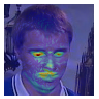
\includegraphics[width=.16\linewidth]{img/saliency_smoothgrad/saliency_1Lip_3_crop.png} &
  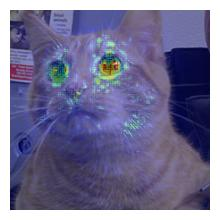
\includegraphics[width=.16\linewidth]{img/catvsdog/OTNN_saliency_1.jpg} & 
  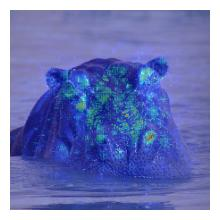
\includegraphics[width=.16\linewidth]{img/imagenet/OTNN_saliency_2.jpg}
  \end{tabular} & 
  \begin{tabular}{@{}l@{}l@{}l@{}}
  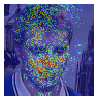
\includegraphics[width=.16\linewidth]{img/saliency_smoothgrad/saliency_Unconst_3_crop.png} &
  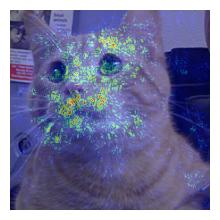
\includegraphics[width=.16\linewidth]{img/catvsdog/resnet50_saliency_1.jpg} & 
  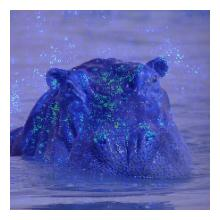
\includegraphics[width=.16\linewidth]{img/imagenet/resnet50_saliency_2.jpg}
  \end{tabular}\\

  \begin{tabular}{l}
   \rotatebox{90}{\textbf{SmoothGrad}} 
  \end{tabular} &
  \begin{tabular}{@{}l@{}l@{}l@{}} 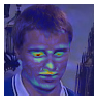
\includegraphics[width=.15\linewidth]{img/saliency_smoothgrad/smoothgrad_1Lip_3_crop.png} &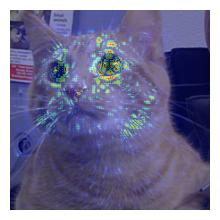
\includegraphics[width=.16\linewidth]{img/catvsdog/OTNN_smooth_1.jpg} & 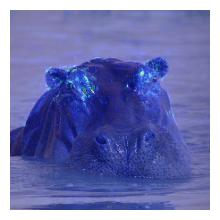
\includegraphics[width=.16\linewidth]{img/imagenet/OTNN_smooth_2.jpg}
  \end{tabular} & 
  \begin{tabular}{@{}l@{}l@{}l@{}}
  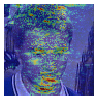
\includegraphics[width=.16\linewidth]{img/saliency_smoothgrad/smoothgrad_Unconst_3_crop.png} & 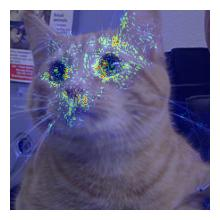
\includegraphics[width=.16\linewidth]{img/catvsdog/resnet50_smooth_1.jpg} & 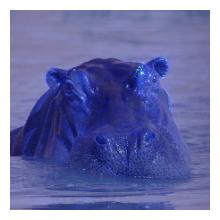
\includegraphics[width=.16\linewidth]{img/imagenet/resnet50_smooth_2.jpg}
  \end{tabular}\\
& (a)~\otnn
  &  (b) Unconstrained
\end{tabular}
\caption{Comparison of Saliency Map and SmoothGrad  explanations for (a) \otnn~ and (b) unconstrained network for, from left to right, CelebA, Cat vs Dog and Imagenet datasets.} %\commentgreen{Thomas a donné des nouvelles images elles sont dans saliency_smoothgrad/robust... a mettre en annexe ou ici }}
\label{fig:saliency_smoothgrad}
\end{figure*}
\fi

\iffalse
\begin{figure*}
\begin{tabular}{@{}c@{}c@{}c}
\centering
  \begin{tabular}{l}
    \rotatebox{90}{\textbf{Saliency}}
  \end{tabular}
 & 
  \begin{tabular}{@{}l@{}l@{}l}
    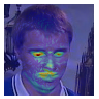
\includegraphics[width=.14\linewidth]{img/saliency_smoothgrad/saliency_1Lip_3_crop.png} &
  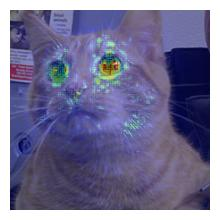
\includegraphics[width=.15\linewidth]{img/catvsdog/OTNN_saliency_1.jpg} %& 
%  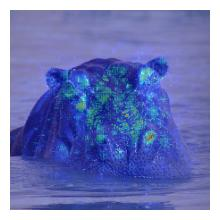
\includegraphics[width=.15\linewidth]{img/imagenet/OTNN_saliency_2.jpg}
  \end{tabular} &
  \multirow{6}{c}{\includegraphics[width=.35\textwidth]{img/human_alignment.jpg}}
  \\

  \begin{tabular}{l}
   \rotatebox{90}{\textbf{SmoothGrad}} 
  \end{tabular} &
  \begin{tabular}{@{}l@{}l@{}l} 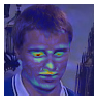
\includegraphics[width=.14\linewidth]{img/saliency_smoothgrad/smoothgrad_1Lip_3_crop.png} &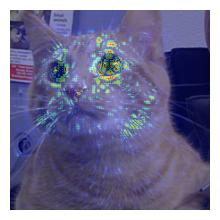
\includegraphics[width=.15\linewidth]{img/catvsdog/OTNN_smooth_1.jpg} %& 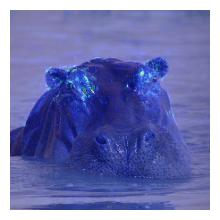
\includegraphics[width=.15\linewidth]{img/imagenet/OTNN_smooth_2.jpg}
  \end{tabular} &  \\
& (a)~\otnn  & \\
  \begin{tabular}{l}
    \rotatebox{90}{\textbf{Saliency}}
  \end{tabular}
 & 
  \begin{tabular}{@{}l@{}l@{}l}
  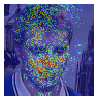
\includegraphics[width=.15\linewidth]{img/saliency_smoothgrad/saliency_Unconst_3_crop.png} &
  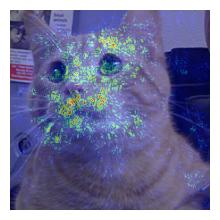
\includegraphics[width=.16\linewidth]{img/catvsdog/resnet50_saliency_1.jpg} %& 
%  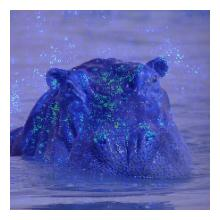
\includegraphics[width=.15\linewidth]{img/imagenet/resnet50_saliency_2.jpg}
  \end{tabular}  & \\
  \begin{tabular}{l}
   \rotatebox{90}{\textbf{SmoothGrad}} 
  \end{tabular} &
  \begin{tabular}{@{}l@{}l@{}l}
  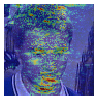
\includegraphics[width=.15\linewidth]{img/saliency_smoothgrad/smoothgrad_Unconst_3_crop.png} & 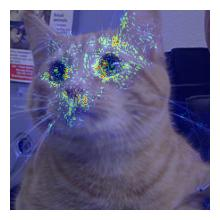
\includegraphics[width=.16\linewidth]{img/catvsdog/resnet50_smooth_1.jpg} %& 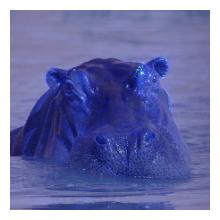
\includegraphics[width=.15\linewidth]{img/imagenet/resnet50_smooth_2.jpg}
  \end{tabular} & \\
&   (b) Unconstrained& 
\end{tabular}
\caption{Comparison of Saliency Map and SmoothGrad  explanations for (a) \otnn~ and (b) unconstrained network for the respectively CelebA, cat vs dog and imagenet.} %\commentgreen{Thomas a donné des nouvelles images elles sont dans saliency_smoothgrad/robust... a mettre en annexe ou ici }}
\label{fig:saliency_smoothgrad}
\end{figure*}
\fi
%\textbf{Saliency Map on \otnn~are less complex:} 
%Complexity of a given explanation is linked to the understandability by a human. \commentgreen{Thomas si tu as des references ? TBC should be kolmogorov but JPEG is a good surrogate}
%Inspired by previous works~\cite{da2011image} highlighting a strong correlation between Kolmogorov complexity and human evaluation of complexity~\cite{forsythe2008confounds,forsythe2009visual}. We used a JPEG based compressor~\cite{vereshchagin2005lossy} as a simple approximation of  visual explanation complexity~\cite{li2004similarity}: \otnn s~yield simpler explanations than unconstrained networks in all case. %($16.8kB$) -see Figure~\ref{fig:saliency_smoothgrad} for a qualitative comparison-.
%. \commentgreen{il manque les resultats (a faire Franck)}



%\subsubsection{\otnn s~ provide better explanations}
%\commentgreen{idem better ca veut pas dire grand chose\\
%\otnn s~ explanations exhibit more fidelity and stability\\
%...\\
%d'autres propositions?}





\textbf{\otnn s~ explanations are aligned with human ones : }
Adopting the method presented in~\cite{linsley2017visual}, using the ClickMe dataset, we follow strictly their experimental methodology and use their code\footnote{https://github.com/serre-lab/Harmonization} to compute the human feature alignment of OTNN Saliency Maps and compare with the others models tested in ~\cite{ fel2022aligning}-- more than 100 recent deep neural networks. In Figure ~\ref{fig:human_alignement}, we demonstrate that 
OTNN models Saliency Maps, %the Saliency Map of  the OTNN model,
which also carries a theoretical interpretation as the direction of the transport plan,  is more aligned with human attention than any other tested models and significantly surpasses the Pareto front discovered by~\cite{fel2022aligning}. The OTNN model is even more aligned than a ResNet50 model trained with a specific alignment objective, proposed by~\cite{fel2022aligning}, and called \textit{Harmonized ResNet50}. 
This finding is interesting as it indicates \otnn s are less prone to relying on spurious correlations~\cite{geirhos2020shortcut} and 
%is more adept at capturing 
better capture
human visual strategies for object recognition.
%The implications of these findings are crucial first for cognitive science: A model with closer alignment with human attention and visual strategies can provide a more comprehensive understanding of how vision operates for humans. Besides, it enhances the predictability, interpretability, and performance of object recognition models which as positive consequences in industry settings.
The implications of these results are crucial for both cognitive science and industrial applications. A model that more closely aligns with human attention and visual strategies can provide a more comprehensive understanding of how vision operates for humans, and also enhance the predictability, interpretability, and performance of object recognition models in industry settings. 
Furthermore, the drop in alignment observed in recent models highlights the necessity of considering the alignment of model visual strategies with human attention while developing object recognition models to reduce the reliance on spurious correlations and ensure that our models get things right for the right reasons.

\iftrue
\begin{figure*}
\centering
\includegraphics[width=1.\textwidth]{img/human_alignment_flat_2.pdf}
\caption{\textbf{\otnn~are aligned with Human attention.} Our study shows that the Saliency Map of OTNN model is highly aligned with human attention.% This finding is supported by the work of~\cite{fel2022aligning}, which demonstrates the trade-off between deep neural network (DNN) performance and alignment with human feature importance from the ClickMe~\cite{linsley2017visual} dataset. The degree of alignment between human and DNN saliency is measured using the mean Spearman correlation, normalized by the average inter-rater alignment of humans. 
%Among the hundreds of model tests performed in the original study, our model is the only one that breaks the Pareto front, suggesting a superior trade-off between DNN performance and alignment with human attention. Even an Harmonized model from~\cite{fel2022aligning} study, which was specifically designed to predict human attention, achieves a lower alignment than our model. \fel{on peut remove ca si vous voulez:} Overall, our results highlight the potential of the OTNN model to capture the visual strategies used by humans for object recognition, and may lead to improved performance and interpretability of object recognition models in both cognitive science and industry applications.
}
\label{fig:human_alignement}
\end{figure*}
\fi



\iffalse
\begin{figure*}
\centering
\includegraphics[width=.7\textwidth]{img/human_alignment.jpg}
\caption{\textbf{\otnn~are aligned with Human attention.} Our study shows that the Saliency Map of \otnn~model is highly aligned with human attention.% This finding is supported by the work of~\cite{fel2022aligning}, which demonstrates the trade-off between deep neural network (DNN) performance and alignment with human feature importance from the ClickMe~\cite{linsley2017visual} dataset. The degree of alignment between human and DNN saliency is measured using the mean Spearman correlation, normalized by the average inter-rater alignment of humans. 
%Among the hundreds of model tests performed in the original study, our model is the only one that breaks the Pareto front, suggesting a superior trade-off between DNN performance and alignment with human attention. Even an Harmonized model from~\cite{fel2022aligning} study, which was specifically designed to predict human attention, achieves a lower alignment than our model. \fel{on peut remove ca si vous voulez:} Overall, our results highlight the potential of the OTNN model to capture the visual strategies used by humans for object recognition, and may lead to improved performance and interpretability of object recognition models in both cognitive science and industry applications.
}
\label{fig:human_alignement}
\end{figure*}
\fi
%Reseau normal: Grad => metriques nulles; comparer avec autre methode d'explication
%Reseau hKR: Grad => metriques++; eventuellement comparer autres explications 
%Metriques: robustnes-Sr; stability; .... (voir avec thomas les autres potentiellement deja dans xplique qu'on pourrait tester )
%\subsection{adult} explaination show unfairness

%\subsection{Qualitative results}
\textbf{Qualitative results: }
Using the learnt \otnn~on FashionMNIST, CelebA (Mouth Slightly Open label), Cat vs Dog and Imagenet, Fig.~\ref{fig:celebA_counterfactual},\ref{fig:fashionMNIST_counterfactual}  present the original image, average gradients $\nabla_x f_j$  over the channels, and images in the direction of the transport plan (Prop.~\ref{th:gradient_transport_plan}), other samples are given in Appendix~A.5. 
We can see that most of the gradients are visually consistent, showing clearly what has to be changed in the input image to modify the class and act as a counterfactual explanation. 
%what needed to change in the input image to classes and act as a counterfactual explanation. 
This is less clear for the Imagenet examples. This could be due to the difficulty of defining a transport plan for each pair of the 1000 classes. However, feature visualizations in Figure \ref{fig:big_picture} show that the internal representation of the classes is still more interpretable than the unconstraint one. 
More generally, we observe that the gradient gives clear information about how the classifier makes its decision. For instance, for the cat, it shows that the classifier does not need to encode perfectly the concept of a cat, but mainly to identify the color of the eyes and size of the nose.
%\commentgreen{@Mathieu tu en feras d'autres images sinon enlever la paranthese}

\iffalse
\begin{figure*}
    \centering
        \begin{tabular}{ccc}
        \multicolumn{3}{c}{CelebA Mouth Slightly Open label: left close to open, right open to close} \\
        \begin{tabular}{ccc}
            \includegraphics[width=.13\linewidth]{img/Mouth_slightly_open/00024_input_lbl0_fx-0.59.pdf} & \includegraphics[width=.13\linewidth]{img/Mouth_slightly_open/00024_gradColor.pdf} & \includegraphics[width=.13\linewidth]{img/Mouth_slightly_open/00024_xMinus10.0Grad.pdf} 
        \end{tabular} &
        \begin{tabular}{ccc}
            \includegraphics[width=.13\linewidth]{img/Mouth_slightly_open/00072_input_lbl1_fx0.47.pdf} & \includegraphics[width=.13\linewidth]{img/Mouth_slightly_open/00072_gradColor.pdf} & \includegraphics[width=.13\linewidth]{img/Mouth_slightly_open/00072_xMinus10.0Grad.pdf} 
        \end{tabular} & \\
         %\midrule
          
        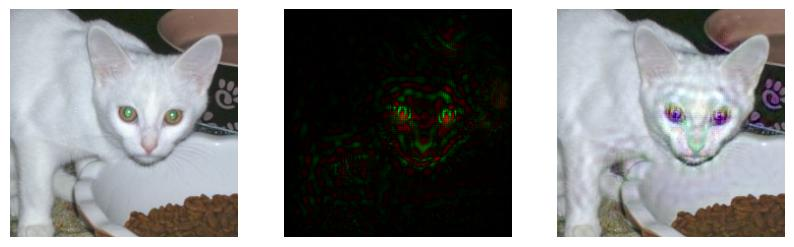
\includegraphics[width=.5\linewidth] {img/catvsdog/expl_1.jpg} &
        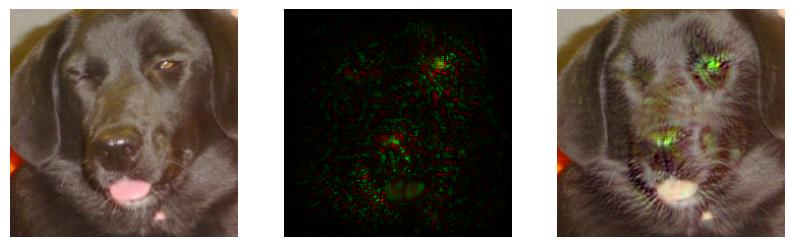
\includegraphics[width=.5\linewidth] {img/catvsdog/expl_2.jpg} & \\
        % \midrule
        \multicolumn{3}{c}{Imagenet :left cabbage butterfly to monarch one,  right great grey owl to bald eagle} \\
        
\includegraphics[width=.5\linewidth] {img/imagenet/expl_1.jpg} &
        
\includegraphics[width=.5\linewidth] {img/imagenet/expl_2.jpg} %\\
        & \\
     \end{tabular}
    \caption{Samples of conterfactuals from different dataset: (left) source image , (center) gradient image, (right) counterfactual of the form $\x-t*\hat{f}(\x)\nabla_x \hat{f}(\x)$, for  $t>1$}
    \label{fig:celebA_counterfactual}
\end{figure*}


\begin{figure*}[h]
  \centering
  \fbox{\includegraphics[width=0.98\linewidth]{img/fashion-otnn.png}}
  
\caption{Samples from different classes of FashionMNIST: (left) source image , (center) targeted gradient image of an \otnn, (right) targeted counterfactual of the form $\x-10*\hat{f}(\x)\nabla_x \hat{f}(\x)$}
%Counterfactuals of the form $ \x-10*\hat{f}(\x)\nabla_x \hat{f}(\x)$  of a \otnn~ for FashionMNIST. }
\label{fig:fashion_mnist}
\end{figure*}
\fi


\begin{figure*}
\centering
\begin{tabular}{ccc}
%\multicolumn{3}{c}{Fashion MNIST source image and class, targeted gradient image and counterfactual.} \\
\multicolumn{3}{c}{\includegraphics[width=1.0\linewidth]{img/fashion-otnn.pdf}}\\
\end{tabular}
\caption{Samples of counterfactuals for FashionMNIST dataset on different classes and targets: (left) source image , (center) gradient image, (right) counterfactual of the form $\x-t*\hat{f}(\x)\nabla_x \hat{f}(\x)$, for  $t>1$}
\label{fig:fashionMNIST_counterfactual}
\end{figure*}

\iftrue
\begin{figure*}
    \centering
    \begin{tabular}{rcc}
        %\multicolumn{3}{c}{Fashion MNIST source image and class, targeted gradient image and counterfactual.} \\
        %\multicolumn{3}{c}{\includegraphics[width=1.0\linewidth]{img/fashion-otnn.pdf}}\\
        %\multicolumn{3}{c}{CelebA Mouth Slightly Open label: left close to open, right open to close} \\
        \rotatebox[origin=c]{90}{CelebA}\hspace{-5mm} & 
        \begin{tabular}{ccc}
            \includegraphics[width=.13\linewidth]{img/Mouth_slightly_open/00024_input_lbl0_fx-0.59.pdf} & \includegraphics[width=.13\linewidth]{img/Mouth_slightly_open/00024_gradColor.pdf} & \includegraphics[width=.13\linewidth]{img/Mouth_slightly_open/00024_xMinus10.0Grad.pdf}\\
            % \textbf{mouth closed} & $\to$ & \textbf{mouth opened}
        \end{tabular} &
        \begin{tabular}{ccc}
            \hspace{-4mm}
            \includegraphics[width=.13\linewidth]{img/Mouth_slightly_open/00072_input_lbl1_fx0.47.pdf} & \includegraphics[width=.13\linewidth]{img/Mouth_slightly_open/00072_gradColor.pdf} & \includegraphics[width=.13\linewidth]{img/Mouth_slightly_open/00072_xMinus10.0Grad.pdf} \\
            % \textbf{mouth opened} & $\to$ & \textbf{mouth closed}
        \end{tabular} \\
          & \textbf{mouth closed $\to$ mouth opened} &  \textbf{mouth opened $\to$ mouth closed}\\
        %\midrule
        % \multicolumn{3}{c}{CelebA Blurry label: left blurry to not blurry, right not blurry to blurry} \\
        %%%%%%%%%%%%%%%%%%%%%%%%%
        \rotatebox[origin=c]{90}{CelebA}\hspace{-5mm} & 
        \begin{tabular}{ccc}
            \includegraphics[width=.13\linewidth]{img/samplesAppendix/Blurry/00027_input_lbl1_fx0.72.pdf} & \includegraphics[width=.13\linewidth]{img/samplesAppendix/Blurry/00027_gradColor.pdf} & \includegraphics[width=.13\linewidth]{img/samplesAppendix/Blurry/00027_xMinus10.0Grad.pdf}\\
            % \textbf{blurry} & $\to$ & \textbf{not blurry}
        \end{tabular} &
        \begin{tabular}{ccc}
            \hspace{-4mm}
            \includegraphics[width=.13\linewidth]{img/samplesAppendix/Blurry/00250_input_lbl0_fx-1.15.pdf} & \includegraphics[width=.13\linewidth]{img/samplesAppendix/Blurry/00250_gradColor.pdf} & \includegraphics[width=.13\linewidth]{img/samplesAppendix/Blurry/00250_xMinus5.0Grad.pdf}\\
            % \textbf{not blurry} & $\to$ & \textbf{blurry}
        \end{tabular} \\
          & \textbf{blurry $\to$ not blurry} & \textbf{not blurry $\to$ blurry}\\
        %\midrule
        % \multicolumn{3}{c}{CelebA Rosy cheeks label: rosy to not rosy, right not rosy to rosy} \\
        %%%%%%%%%%%%%%%%%%%%%%%%%%%%%%%%%%%%%
        \rotatebox[origin=c]{90}{CelebA}\hspace{-5mm} & 
        \begin{tabular}{ccc}
            \includegraphics[width=.13\linewidth]{img/samplesAppendix/Rosy_Cheeks/00132_input_lbl1_fx3.26.pdf} & \includegraphics[width=.13\linewidth]{img/samplesAppendix/Rosy_Cheeks/00132_gradColor.pdf} & \includegraphics[width=.13\linewidth]{img/samplesAppendix/Rosy_Cheeks/00132_xMinus2.5Grad.pdf}\\
            % \textbf{rosy cheeks} & $\to$ & \textbf{w/o rosy cheeks}
        \end{tabular} &
        \begin{tabular}{ccc}
            \hspace{-4mm}
            \includegraphics[width=.13\linewidth]{img/samplesAppendix/Rosy_Cheeks/00079_input_lbl0_fx-7.52.pdf} & \includegraphics[width=.13\linewidth]{img/samplesAppendix/Rosy_Cheeks/00079_gradColor.pdf} & \includegraphics[width=.13\linewidth]{img/samplesAppendix/Rosy_Cheeks/00079_xMinus2.0Grad.pdf}\\
            % \textbf{w/o rosy cheeks} & $\to$ & \textbf{rosy cheeks}
        \end{tabular} \\
        & \textbf{rosy cheeks $\to$ w/o rosy cheeks} & \textbf{w/o rosy cheeks $\to$ rosy cheeks}\\
        %\midrule 
        %\multicolumn{3}{c}{Cat vs dog : left cat to dog, right dog to cat} \\
        \rotatebox{90}{\quad Cat vs Dog}\hspace{-5mm} &
        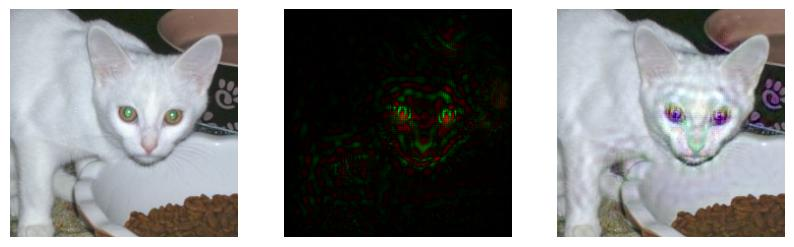
\includegraphics[width=.464\linewidth] {img/catvsdog/expl_1.jpg} &
            \hspace{-4mm}
        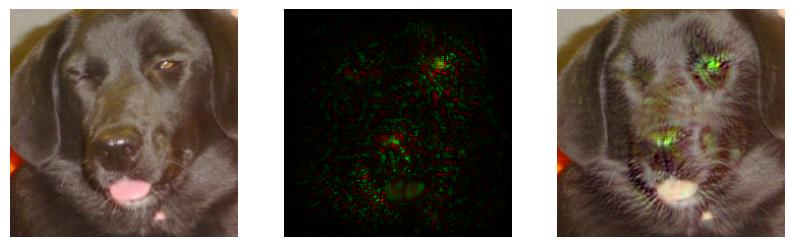
\includegraphics[width=.464\linewidth] {img/catvsdog/expl_2.jpg}\\
        & \textbf{cat $\to$ dog} & \textbf{dog $\to$ cat}\\
        % \midrule
        % \multicolumn{3}{c}{Imagenet :left cabbage butterfly to monarch one,  right great grey owl to bald eagle} \\
        \rotatebox{90}{\quad Imagenet}\hspace{-5mm} &
        
\includegraphics[width=.464\linewidth] {img/imagenet/expl_1.jpg} &
            \hspace{-4mm}
        
\includegraphics[width=.464\linewidth] {img/imagenet/expl_2.jpg} \\
        & \textbf{cabbage butterfly $\to$ monarch butterfly} & \textbf{great grey owl $\to$ bald eagle}\\
     \end{tabular}
    \caption{Samples of counterfactuals from different datasets: (left) source image , (center) gradient image, (right) counterfactual of the form $\x-t*\hat{f}(\x)\nabla_x \hat{f}(\x)$, for  $t>1$}
    \label{fig:celebA_counterfactual}
\end{figure*}
\fi



\section{Conclusions and broader impact}
In this paper, we study the explainability properties of OTNN~(Optimal Transport Neural Networks) 
that are 1-Lipschitz~constrained neural networks trained with an optimal transport dual loss. 
We establish that the gradient of the optimal solution aligns with the transportation plan direction,
and the closest decision boundary point (adversarial example) also lies in this gradient direction at a distance of the absolute value of the network output.  
Relying on a formal definition of Optimal Transport counterfactuals, we build a link between the OTNN gradients and counterfactual explanations
%, justifying that 
. We thus show that
OTNNs loss jointly targets the classification task and induces a gradient alignment to the transportation plan. 
%building a counterfactual explanation. 
These beneficial properties of the gradient substantially enhance the Saliency Map XAI method for \otnn~s.
The experiments show that the simple Saliency Map has top-rank scores on state-of-the-art XAI metrics, and largely outperforms any method applied to unconstrained networks. 
%This is illustrated in the experiments which shows that the simple Saliency Map for OTTNs has top-rank scores on state-of-the-art XAI metrics, and largely outperforms any method applied to unconstrained networks. 
Besides, as far as we know, our models are the first large provable 1-Lipschitz neural models that match state-of-the-art results on large problems.
%To the best of our knowledge, our models are also the first large, provable 1-Lipschitz neural models that achieve results on-par with state-of-the-art on large problems. 
And even if counterfactual explanations are less compelling on Imagenet, probably due to the complexity of transport for 
large number of classes
%multiclass
, we prove that \otnn s Saliency Maps are impressively aligned to human explanations. 
%Last but not least, we prove that \otnn s Saliency Maps are impressively aligned to human explanations. However, counterfactual explanations are less compelling for imagenet. We postulate that the issue of transport for multiple classes is substantially more complex than a mere class distinction, thereby necessitating larger and more adaptable architectures for 1-Lipschitz neural networks.


\textbf{Broader impact.} This paper demonstrates the value of OTNNs~for critical problems. OTNNs~are certifiably robust and explainable with the simple Saliency Map method (highly aligned with human explanations) and have accuracy performances comparable to unconstrained networks.% On the other hand, even if the learning process of these networks is between 3 and 6 times longer than for unconstrained ones, at the inference time, OTNNs~are classical networks with the same computation cost as their unconstrained counterparts. 
Though OTNNs take 3-6 times longer to train than unconstrained networks, they have similar computational costs during inference.
We hope that this contribution will raise a great interest in these OTNN networks.

%We first provide  enhancements of the \losshkr, proposed in\cite{serrurier2021achieving}, reducing the number of hyperparameters and the improving the performances at convergence. 
%Experiments provide quantitative and qualitative evaluations showing that Saliency Maps for OTNNs have better score than for unconstrained networks, and comparable scores to other XAI methods.To end with we show that Saliency Maps for OTNNs have an unprecedented alignment to human explanations.   
%OTNNs, because of their connection with optimal transport, structurally produce counterfactual explanations. Indeed, we prove that the gradient of an OTNN at a point represents the direction of the adversarial attack but also of its image in the optimal transport plan, transforming the adversary attacks into an understandable counterfactual explanation.  
%This is illustrated in the experiment which shows that the simple Saliency Map for OTTNs has top-rank scores on state-of-the-art XAI metrics, and largely outperforms any method applied to unconstrained networks.\commentgreen{Last but not least, we prove that \otnn s Saliency Maps are impressively aligned to human explanations.} 

%\commentgreen{peut etre renommer pour ne pas trop faire post neurips, et developper les points negatifs de notre methode -voir reponse au reviewer-}


\begin{ack}
This work has benefited from the AI Interdisciplinary Institute ANITI, which is funded by the French ``Investing for the Future – PIA3'' program under the Grant agreement ANR-19-P3IA-0004. The authors gratefully acknowledge the support of the DEEL project.\footnote{\url{https://www.deel.ai/}}
\end{ack}

\bibliographystyle{abbrv} %plainnat
\bibliography{hkr_explainability}
%%%%%%%%%%%%%%%%%%%%%%%%%%%%%%%%%%%%%%%%%%%%%%%%%%%%%%%%%%%%s

%\newpage
%\input{parts/checklist}

%%%%%%%%%%%%%%%%%%%%%%%%%%%%%%%%%%%%%%%%%%%%%%%%%%%%%%%%%%%%
\newpage

\appendix

\section{Appendix}
\subsection{Additional definition and proofs}
\label{ann:def_and_proof}
Let us first recall the optimal transport problem associated with the minimization of \losshkr:
\begin{equation}\label{eq:dual}
\underset{f\in Lip_1(\Omega)} {\inf} \mathcal{L}^{hKR}_{\lambda(f),m} = \inf_{\pi \in\Pi^p_{\lambda}(\dpos, \dneg)}\int_{\Omega\times \Omega}|{\x}-{{\z}} |d\pi + \pi_{\x}(\Omega)+\pi_{{\z}}(\Omega)-1
\end{equation}
Where $\Pi^p_{\lambda}(\dpos, \dneg)$ is the set consisting of positive measures $\pi\in \mathcal{M}_+(\Omega\times \Omega)$ which  are absolutely continuous with respect to the joint measure $d\dpos\times d\dneg$ and $\frac{d\pi_{\textbf{x}}}{d\dpos}\in [p, p(m+\lambda)]$, $\frac{d\pi_{{\textbf{z}}}}{d\dneg}\in [1-p, (1-p)(m+\lambda)] $.
We name $\pi^*$  the optimal transport plan according to Eq.\ref{eq:dual} and and $f^*$ the associated potential function.

\textbf{Proof of proposition 1}:
According to \cite{serrurier2021achieving}, we have 
$$ ||\nabla_x f^*(\x)||=1 $$
almost surely and

$$\mathbb{P}_{(\x,\y)\sim\pi^*} \left( |f^*(\x) - f^*(\y)| = ||\x - \y|| \right)=1$$
Following the proof of proposition 1 in \cite{gulrajani2017improved} and \cite{Ambrosio2003} we have :\\
Given $\x_\alpha = \alpha*x + (1-\alpha) \y$, $0\leq\alpha\leq1$
$$ \mathbb{P}_{(\x,\y)\sim\pi^*} \left( \nabla_x f^*(\x_\alpha) =\frac{\x_\alpha - \y}{ ||\x_\alpha - \y||} \right)=1.$$
So for for $\alpha = 1$ whe have
$$ \mathbb{P}_{(\x,\y)\sim\pi^*} \left( \nabla_x f^*(\x) =\frac{\x - \y}{ ||\x - \y||} \right)=1$$
and then 
$$ \mathbb{P}_{(\x,\y)\sim\pi^*} \left( \y = \x -  \nabla_x f^*(\x) .||\x - \y|| \right)=1$$
This prove the proposition 1 by choosing $t=||\x - \y||$.\BlackBox\\

\textbf{Proof of proposition 2}:
Let $\dpos$ and $\dneg$ two distributions with disjoint support with minimal distance~$\epsilon$ and  $f^*$ an optimal solution minimizing the \losshkr~with $m<2\epsilon$. According to \cite{serrurier2021achieving}, $f^*$ is $100\%$ accurate. Since the classification is based on the sign of f we have : $\forall \x \in \dpos, f^*(\x) \geq 0$ and $\forall \y \in \dneg, f^*(\y) \leq 0$. Given $\x \in \dpos$ and $\y = tr_\pi(\x) = \x  -t \nabla_x f^*(\x)$  and $\y \in  \dneg$. According to the previous proposition we have :
\begin{align*}
  |f^*(\x) - f^*(\y)| & =||\x -\y || & \\
 |f^*(\x) - f^*(\y)| & =||\x -(\x  -t \nabla_x f^*(\x) ) || &\\
 |f^*(\x) - f^*(\y)| & =||t \nabla_x f^*(\x) ) || &\\
 |f^*(\x) - f^*(\y)| & =t.|| \nabla_x f^*(\x) ) || & (t\geq 0)\\
 |f^*(\x) - f^*(\y)| & =t & (\nabla_x f^*(\x) = 1)\\
 f^*(\x) - f^*(\y) & =t & (f^*(\x) \geq 0,f^*(\y) \leq 0) \\
 f^*(\y) & =f^*(\x) - t & 
\end{align*}
since $f^*(\y)\leq 0$ we obtain :
$$f^*(\x) \leq t $$
Since $f^*$ is continuous, $\exists t'>0$ such that $ \x_\delta = \x  -t' \nabla_x f^*(\x) $ and $f^*(\x_\delta) = 0$. We have :
\begin{align*}
|f^*(\x) - f^*(\x_\delta|) & \leq ||\x -\x_\delta || & \\
f^*(\x) &\leq||\x -(\x  -t' \nabla_x f^*(\x) ) || &\\
f^*(\x) &\leq t'&
\end{align*}
and 
\begin{align*}
|f^*(\x_\delta) - f^*(\y)| & \leq ||\x_\delta -\y|| & \\
-f^*(\y) &\leq||(\x  -t' \nabla_x f^*(\x) )  - (\x  -t \nabla_x f^*(\x))|| &\\
-f^*(\y) &\leq t-t'&\\
-f^*(\y) &\leq ||\x-\y ||-t'& )\\
\end{align*}
Then, if $f^*(\x) < t'$ we have
\begin{align*}
f^*(\x)-f^*(\y) < &t'+||\x-\y ||-t' \\
f^*(\x)-f^*(\y) < &||\x-\y || \\
\end{align*}
which is a contradiction so $f^*(\x) = t'$ and
$$\x_\delta = \x  -f^*(\x) \nabla_x f^*(\x) $$
\BlackBox

\newpage 

\subsection{Parameters and architectures}
\label{ann:parameters}
\subsubsection{Datasets}

\textbf{FashionMNIST} has 50,000 images for training and 10,000 for test of size $28 \times 28 \times 1$, with 10 classes.

\textbf{CelebA} contains 162,770 training samples, 19,962 samples for test of size $218\times 178 \times 3$. We have used  a subset of 22 labels: \textit{Attractive}, \textit{Bald}, \textit{Big\_Nose},
\textit{Black\_Hair}, \textit{Blond\_Hair}, \textit{Blurry}, \textit{Brown\_Hair}, \textit{Eyeglasses}, \textit{Gray\_Hair}, \textit{Heavy\_Makeup}, \textit{Male}, \textit{Mouth\_Slightly\_Open}, \textit{Mustache}, \textit{Receding\_Hairline}, \textit{Rosy\_Cheeks}, \textit{Sideburns}, \textit{Smiling}, \textit{Wearing\_Earrings}, \textit{Wearing\_Hat}, \textit{Wearing\_Lipstick}, \textit{Wearing\_Necktie}, \textit{Young}.

Note that labels in CelebA are very unbalanced (see~Table~\ref{tab:celebA_stats}, with less than $5\%$ samples for \textit{Mustache} or \textit{Wearing\_Hat} for instance). Thus we will use Sensibility and Specificity as metrics.
\begin{table}[h]
  \caption{CelebA label distribution: proportion of positive samples in training set (testing set) [bold: very unbalanced labels]}
  \label{tab:celebA_stats}
  \centering
  \begin{tabular}{c@{}c@{}c@{}c@{}c}
    \toprule
    \textit{Attractive}& \textit{Bald}& \textit{Big\_Nose}&
\textit{Black\_Hair}& \textit{Blond\_Hair}\\
  0.51 (0.50) & \textbf{0.02 (0.02)} & \textbf{0.24 (0.21)} & \textbf{0.24 (0.27)} & \textbf{0.15 (0.13)}  \\
  \textit{Blurry}  & \textit{Brown\_Hair}& \textit{Eyeglasses}& \textit{Gray\_Hair}& \textit{Heavy\_Makeup} \\
 \textbf{0.05 (0.05)} & \textbf{0.20 (0.18)} & \textbf{0.06 (0.06)} & \textbf{0.04 (0.03)} & 0.38 (0.40)  \\
    \textit{Male} & \textit{Mouth\_Slightly\_Open}& \textit{Mustache}& \textit{Receding\_Hairline}& \textit{Rosy\_Cheeks}\\
 0.42 (0.39) & 0.48 (0.50) & \textbf{0.04 (0.04)} & \textbf{0.08 (0.08)} & \textbf{0.06 (0.07)}  \\
    \textit{Sideburns}& \textit{Smiling} & \textit{Wearing\_Earrings}& \textit{Wearing\_Hat}& \textit{Wearing\_Lipstick}\\
    \textbf{0.06 (0.05)} & 0.48 (0.50) & \textbf{0.19 (0.21)} & \textbf{0.05 (0.04)} & 0.47 (0.52)  \\
    \textit{Wearing\_Necktie}& \textit{Young} \\
    \textbf{0.12 (0.14)} &  0.78 (0.76)\\
    \midrule
  \end{tabular}
\end{table}

\textbf{Cat vs Dog} contains 17400 training samples, 5800 test samples of various size. 

\textbf{Imagenet} contains 1M training samples, 100 000 samples for test of various size. 

%*Dataset preprocessing
\paragraph*{preprocessing:}
For FashionMNIST Images are normalized between $[0,1]$ with no augmentation. For CelebA dataset, data augmentation is used with random crop, horizontal flip, random brightness, and random contrast. For imagenet and cat vs dog we use the standart preprocessing of resnet (with no normalization in  $[0,1]$)




\subsubsection{Architectures}
As indicated in the paper, linear layers for \otnn~and unconstrained networks are equivalent (same number of layers and neurons), but unconstrained networks use batchnorm and ReLU layer for activation, whereas \otnn~only use GroupSort2~\cite{pmlr-v97-anil19a,serrurier2021achieving} activation. \otnn~are built using \Deellip library.
%*Loss


    \paragraph*{\onlyonelip~ networks parametrization.} Several soltutions have been proposed to set the Lipschitz constant of affine layers: Weight clipping~\cite{Arjovsky2017} (WGAN), Frobenius normalization~\cite{SalimansK16} and spectral normalization~\cite{Miyato2018SpectralNF}. In order to avoid  vanishing gradients, orthogonalization can be done using Bj{\"o}rck algorithm~\cite{bjorck71Ortho}. DEEL.LIP implements most of these solutions, but we focus on layers called \textit{SpectralDense} and \textit{SpectralConv2D}, with  spectral normalization~\cite{Miyato2018SpectralNF} and  Bj{\"o}rck algorithm~\cite{bjorck71Ortho}.
    Most activation functions are Lipschitz, including ReLU, sigmoid, but we use GroupSort2 proposed by \cite{pmlr-v97-anil19a}, and defined by the following equation:
    $$\text{GroupSort2}(x)_{2i,2i+1}=[\min{(x_{2i},x_{2i+1})},\max{(x_{2i},x_{2i+1})}]$$

Network architectures used for CelebA dataset are described in Table~\ref{tab:NN_archi_celebA}.
\begin{table}[h]
  \caption{CelebA Neural network architectures: Sconv2D is SpectralConv2D, GS2 is GroupSort2, L2Pool is L2NormPooling, SDense is SpectralDense, BN is BatchNorm, AvgPool is AveragePooling}
  \label{tab:NN_archi_celebA}
  \centering
  \begin{tabular}{llll}
    \toprule
    Dataset & \otnn & Unconstrained NN &                   \\
    \cmidrule(r){2-4}
         & Layer     &  Layer     & Output size  \\
    \midrule
    CelebA & Input   &  Input   & $218\times 178\times 3$     \\
            & SConv2D, GS2    & Conv2D, BN, ReLU   &    $218\times 178\times 16$ $ $   \\
            & SConv2D, GS2  & Conv2D, BN, ReLU   & $218\times 178\times 16$     \\
            & L2Pool  & AvgPool   & $109\times 89\times 16$     \\
            & SConv2D, GS2  & Conv2D, BN, ReLU   & $109\times 89\times 32$      \\
            & SConv2D, GS2  &  Conv2D, BN, ReLU  & $109\times 89\times 32$     \\
            & L2Pool  &  AvgPool  & $54\times 44\times 32$     \\
            & SConv2D, GS2  & Conv2D, BN, ReLU   & $54\times 44\times 64$      \\
            & SConv2D, GS2  & Conv2D, BN, ReLU   & $54\times 44\times 64$      \\
            & SConv2D, GS2  & Conv2D, BN, ReLU   & $54\times 44\times 64$      \\
            & L2Pool  & AvgPool   & $27\times 22\times 64$      \\
            & SConv2D, GS2  & Conv2D, BN, ReLU   & $27\times 22\times 128$      \\
            & SConv2D, GS2  & Conv2D, BN, ReLU   & $27\times 22\times 128$      \\
            & SConv2D, GS2  & Conv2D, BN, ReLU   & $27\times 22\times 128$      \\
            & L2Pool  & AvgPool   & $13\times 11\times 128$      \\
            & SConv2D, GS2  & Conv2D, BN, ReLU   & $13\times 11\times 128$      \\
            & SConv2D, GS2  & Conv2D, BN, ReLU   & $13\times 11\times 128$     \\
            & SConv2D, GS2  & Conv2D, BN, ReLU   & $13\times 11\times 128$      \\
            & L2Pool  & AvgPool   & $6\times 5\times 128$      \\
            & Flatten, SDense, GS2  & Flatten, Dense, BN, ReLU & $256$     \\
            & SDense, GS2  & Dense,BN, ReLU    & $256$     \\
            & SDense  & Dense   & $22$    \\
    \bottomrule
  \end{tabular}
\end{table}





Network architectures used for FashionMNIST dataset are described in Table~\ref{tab:NN_archi_Fashion}. The same \otnn~architecture is used for MNIST expermentation presented in Fig.~\ref{fig:big_picture}.

The 1-Lipschitz version of resnet50 is described in Table~\ref{tab:resnetLIP}. As the unconstrained version, It has around 25M parameters. For the large version, we simply multiply the number channels in hidden layers by $1.5$. The unconstrained version is the standart resnet50 architecture. In the case of imagenet we use the pretrained version provided by tensorflow.
\begin{table}[h]
  \caption{FashionMNIST Neural network architectures: Sconv2D is SpectralConv2D, GS2 is GroupSort2, SDense is SpectralDense, BN is BatchNorm, AvgPool is AveragePooling, SGAvgPool is ScaledGlobalAveragePooling (DEEL.LIP), GAvgPool is GlobalAveragePooling}
  \label{tab:NN_archi_Fashion}
  \centering
  \begin{tabular}{llll}
    \toprule
    Dataset & \otnn & Unconstrained NN &                   \\
    \cmidrule(r){2-4}
         & Layer     &  Layer     & Output size  \\
    \midrule
    FashionMNIST & Input   & Input   & $28\times 28\times 1 $     \\  
    & SConv2D, GS2    & Conv2D, BN, ReLU   &    $28\times 28\times 96$   \\
    & SConv2D, GS2  & Conv2D, BN, ReLU   & $28\times 28\times 96$     \\
    & SConv2D, GS2  & Conv2D, BN, ReLU   & $28\times 28\times 96$     \\
    & SConv2D (stride=2), GS2  & Conv2D (stride=2), BN, ReLU   & $14\times 14\times 96$     \\
    & SConv2D, GS2    & Conv2D, BN, ReLU   &    $14\times 14\times 192$   \\
    & SConv2D, GS2    & Conv2D, BN, ReLU   &    $14\times 14\times 192$   \\
    & SConv2D, GS2    & Conv2D, BN, ReLU   &    $14\times 14\times 192$   \\
    & SConv2D (stride=2), GS2  &  Conv2D (stride=2), BN, ReLU &  $7\times 7\times 192$   \\
    & SConv2D, GS2  & Conv2D, BN, ReLU   & $7\times 7\times 384$      \\
    & SConv2D, GS2  & Conv2D, BN, ReLU   & $7\times 7\times 384$      \\
    & SConv2D, GS2  & Conv2D, BN, ReLU   & $7\times 7\times 384$      \\
    & SGAvgPool  & GAvgPool   & $384$      \\
    & SDense  & Dense   & $10$    \\
    \bottomrule
  \end{tabular}
\end{table}



\begin{table}[h]
\caption{1-lip resnet architecture for Imagenet and cat vs dog: Sconv2D is SpectralConv2D, GS2 is GroupSort2, SDense is SpectralDense, BC is Batchcentering (centeing without normalization), SL2npool is ScaledL2NormPooling2D, SGAvgl2Pool is ScaledGlobalL2NormPooling2D, GAvgPool is GlobalAveragePooling}
\label{tab:resnetLIP}
\centering
\begin{tabular}{ll}
Layer                                    & output                   \\ \hline
Input                                    & $224\times 224\times 3$  \\\hline
SConv2D $7\time7$-64 (stride=2), BC, GS2 & $112\times 112\times 64$ \\ \hline
InvertibleDownSampling                   & $56\times 56\times 256$  \\ \hline
$\begin{bmatrix}
\text{SConv2D } 1\times 1 & 64 & \text{BC, GS2} \\
\text{SConv2D } 3\times 3 & 64 & \text{BC, GS2} \\
\text{SConv2D } 1\times 1 & 256 & \text{BC} \\
\text{add-lip} & &\text{BC, GS2} 
\end{bmatrix}$ $\times 3$                     &   $56\times 56\times 256$                 \\ \hline
 SL2npool       &                 $28\times 28\times 256$         \\ \hline
$\begin{bmatrix}
\text{SConv2D } 1\times 1 & 128 & \text{BC, GS2} \\
\text{SConv2D } 3\times 3 & 128 & \text{BC, GS2} \\
\text{SConv2D } 1\times 1 & 512 & \text{BC} \\
\text{add-lip} & &\text{BC, GS2} 
\end{bmatrix}$ $\times 4$                                      &     $28\times 28\times 512$                    \\ \hline
 SL2npool                          &   $14\times 14\times 512$             \\ \hline
 $\begin{bmatrix}
\text{SConv2D } 1\times 1 & 256 & \text{BC, GS2} \\
\text{SConv2D } 3\times 3 & 256 & \text{BC, GS2} \\
\text{SConv2D } 1\times 1 & 1024 & \text{BC} \\
\text{add-lip} & &\text{BC, GS2} 
\end{bmatrix}$ $\times 6$                                        &     $14\times 14\times 1024$     \\ \hline
 SL2npool                          &   $7\times 7\times 1024    $         \\ \hline
$\begin{bmatrix}
\text{SConv2D } 1\times 1 & 256 & \text{BC, GS2} \\
\text{SConv2D } 3\times 3 & 256 & \text{BC, GS2} \\
\text{SConv2D } 1\times 1 & 1024 & \text{BC} \\
\text{add-lip} & &\text{BC, GS2} 
\end{bmatrix}$ $\times 3$                                         &     $7\times 7\times 2048    $          \\ \hline
    SGAvgl2Pool               &    $2048$   \\ \hline
        SDense                              & $\begin{matrix}
1 & \text{cat vs dog}\\
1000 & \text{imagenet}
\end{matrix}$ 
\end{tabular}
\end{table}



\subsubsection{Losses and optimizer}
An extension of $\mathcal{L}^{hKR}$ to the  multiclass case with $q$ classes. has also been proposed in \cite{serrurier2021achieving}  The idea is to learn $q$ \onlyonelip~functions $f_1, \ldots, f_q$, each component $f_i$ being a  \textit{one-versus-all} binary classifier. The loss proposed was the following 
\begin{equation}
\label{eq:hkr_multi}
\mathcal{L}^{hKR}_{\lambda,m}(f_{1,\ldots,q}) = \sum_{k=1}^q \left[\underset{\textbf{x}  \sim \neg P_k}{\mathbb{E}} \left[f_k(\textbf{x})\right] -\underset{\textbf{x} \sim P_k}{\mathbb{E}}\left[f_k(\textbf{x})\right] \right]
 +\lambda\underset{\textbf{x},\y\sim \underset{k=1}{\bigcup^q}P_k
 }{\mathbb{E}}(H\left(f_1(\x),\ldots, f_q(\x) ,\y,m\right)
\end{equation}
with :
\iftrue
$$
H\left(f_1(\x),\ldots, f_q(\x),\y,m \right) =(m- f_y(\x))_+  + \sum_{k\neq y} (m +f_k(\x))_+
$$
\fi
\iffalse
$$
H\left(f_1(\x),\ldots, f_q(\x),\y,m \right) =\sum_{k=1}^q (m -(2*\mathbb{1}_{y=k}-1)*f_k(\x))_+
$$
\fi
This formulation has three main drawbacks: (i) for large number of classes several outputs may have few or no positive sample within a batch leading to slow convergence, (ii)  weight of $f_y(\x)$ (the function of the true class) with respect to the other decreases when the number of classes increases, (iii) the expectancy has to be evaluated through the batch, making the loss dependant of the size of the batch. 

%To overcome these drawbacks, we propose a sample-wise loss weighted by a softmax :
%\begin{equation}
%\label{eq:hkr_multiv2}
%\begin{split}
%\mathcal{L}^{hKR}_{\lambda,\alpha}(f_{1,\ldots,q},x,y)  &= \left[ \sum_{k\neq y} \left[ f_k(\x)*\frac{e^{\alpha*f_k(\x)}}{\sum_{j\neq y} e^{\alpha*f_j(\x)}}  \right] -f_y(\textbf{x}) \right] \\
%& +\lambda \left[ (m- f_y(\x))_+  + \sum_{k\neq y} \left[\frac{e^{\alpha*f_k(\x)}}{\sum_{j\neq y} e^{\alpha*f_j(\x)}}*(m +f_k(\x))_+\right]\right]
% \end{split}
%\end{equation}
%\fi

\iftrue
To overcome these drawbacks, we propose first to replace the Hinge term $H$ with a softmax weighted version. The softmax on all but true class is defined by:

$$
\sigma(f_k(\x),y,\alpha) = \frac{e^{\alpha*f_k(\x)}}{\sum_{j\neq y} e^{\alpha*f_j(\x)}}
$$
We can define a weighted version of $H$ function:

$$H_{\sigma}\left(f_1(\x),\ldots, f_q(\x),\y ,m,\alpha\right) = (m- f_y(\x))_+  + \sum_{k\neq y} \sigma(f_k(\x),y,\alpha)*(m +f_k(\x))_+
$$
\fi
%\begin{equation}
%soft(f_k(\x)) = \frac{e^{f_k(\x)}}{\sum_{j\neq y} e^{f_j(\x)}}
%\end{equation}

In this function, the value of $f_\y(\x)$ for the true class maintains consistent weight relative to the values of other functions, regardless of the number of classes. $\alpha$ is a temperature parameter. Initially, the softmax behaves like an average as all the values of $f_k$ are close. However, during the learning process, as the values of $|f_k|$ increase, the softmax transitions to function like a maximum. Similarly, if a low value is chosen for $\alpha$ 
%is chosen as a low value
, the softmax behaves as an average, resulting in a one vs all hKR loss. 
By choosing a higher value for $\alpha$, the softmax unbalances the weights. Thus 
%As the value chosen for $\alpha$ increases (and the softmax unbalances the weights), 
the loss persists as a one vs all hKR but incorporates a re-weighting of the opposing classes for each targeted class. 

\iftrue
We also propose a sample-wise and weighted version of the KR part (left term in Eq~\ref{eq:hkr_multi}). to get the proposed loss: 
\begin{equation}
\label{eq:hkr_multiv2}
\begin{split}
\mathcal{L}^{hKR}_{\lambda,m, \alpha}(f_{1,\ldots,q},x,y)  &= \left[ \sum_{k\neq y} \left[ f_k(\x)*\sigma(f_k(\x),y,\alpha)  \right] -f_y(\textbf{x}) \right] \\
& +\lambda*H_{\sigma}\left(f_1(\x),\ldots, f_q(\x),\y, m,\alpha\right) 
 \end{split}
\end{equation}
\fi
It's important to note that this definition only applys to the balanced multiclass case (as in FashionMnist and ImageNet). In the unbalanced scenario, the weight must be rescaled according to the a priori distribution of the classes.




For CelebA, with hyperparameters $\lambda$ is set to 20, and $m=1$. For FashionMNIST, we use  Eq.~\ref{eq:hkr_multiv2},   $\lambda$ is set to $5$,  $\alpha=10$ and $m=0.5$. For cat vs dog $\lambda$ is set to $10$ and $m=18$. For imagenet $\lambda$ is set to $500$,  $\alpha=200$ and $m=0.05$.


%*Optimizer
We train all networks with ADAM optimizer~\cite{Diederik14Adam}. We use a batch size of 128, 200 epochs , and a fixed learning rate $1\mathrm{e}{-2}$ for CelebA. For FashionMNIST we perform 200 epochs with a batch size of 128. We fix the learing rate to $5\mathrm{e}{-4}$ for the 50 first epochs, $5\mathrm{e}{-5}$ for the epochs 50-75, $1\mathrm{e}{-6}$ for the last epochs. For cat vs dog we perform 200 epochs with a batch size of 256. We fix the learing rate to $1\mathrm{e}{-2}$ for the 100 first epochs, $1\mathrm{e}{-3}$ for the epochs 100-150, $1\mathrm{e}{-4}$ for the epochs 150-180 and $1\mathrm{e}{-9}$ for the last epochs. For imagenet we perform 40 epochs with a batch size of 512. We fix the learing rate to $5\mathrm{e}{-4}$ for the 30 first epochs, $5\mathrm{e}{-5}$ for the epochs 30-35, $1\mathrm{e}{-5}$ for the epochs 35-38 and $1\mathrm{e}{-9}$ for the last epochs.

\newpage 

\subsection{Complementary results}
\label{ann:complementary_results}
\subsubsection{FashionMNIST performances and ablation study}

Table~\ref{tab:fashion_results} presents different performance resuts on FashionMNIST. First line is the reference unconstrained network. Second line shows the performances of the new version of \lossreg. Table~\ref{tab:fashion_results} also shows that the new version of the $\mathcal{L}^{hKR}_{\lambda,m,\alpha}$ in the multiclass case  (Eq. \ref{eq:hkr_multiv2})  outperforms the \losshkr defined in~\cite{serrurier2021achieving} (Eq. \ref{eq:hkr_multi}). Obviously, the accuracy enhancement  is obtained at the expense of the robustness. The main interest of this new loss is to provide a wider range in the accuracy/robustness trade-off. 

\begin{table}[h]
  \caption{FashionMNIST accuracy comparison with the different version of multiclass \losshkr. For the fixed margin, we use the one that performs best by parameter tuning (i.e. $m=0.5$) }
  \label{tab:fashion_results}
  \centering
  \begin{tabular}{lc}
    \toprule
 Model &      Accuracy \\
Unconstrained &  88.5\\
  \otnn~ \losshkr multiclass version \cite{serrurier2021achieving} ($\lambda = 10$, $m = 0.5)$& 72.2\\
(Ours) \otnn~$\mathcal{L}^{hKR}_{\lambda,m, \alpha}$  ($\lambda = 10$, $m = 0.5$, $\alpha =10$) (Eq.~\ref{eq:hkr_multiv2})& \textbf{88.6}\\
    \bottomrule
  \end{tabular}
\end{table}

\subsubsection{CelebA performances}
Table~\ref{tab:celebA_results} presents the Sensibility and Specificity for each label reached by Unconstrained network and \otnn. 

As a reminder, given True Positive (TP), True Negative (TN), False Positive (FP), False Negative (FN) samples, Sensitivity (true positive rate or Recall) is defined by:
$$
Sens = \frac{TP}{TP+FN}
$$
Specificity  (true negative rate) is defined by:
$$
Spec = \frac{TN}{TN+FP}
$$

\begin{table}[h]
  \caption{CelebA performance results for unconstrained and \otnn~networks}
  \label{tab:celebA_results}
  \centering
  \begin{tabular}{lcccc}
    \toprule
 Model &      \multicolumn{4}{c}{Metrics: Sensibility/Specificity} \\
 \midrule
    &   \textit{Attractive}& \textit{Bald}& \textit{Big\_Nose}&
\textit{Black\_Hair} \\
 Unconstrained &  \textbf{0.83	/	0.81} &	0.64	/	1.00 &	\textbf{0.65	/	0.87} &	\textbf{0.74	/	0.95} \\
 %\otnn & 0.89	/	0.63 &	\commentgreen{0.02	/	1.00} &	\commentgreen{0.35	/	0.93}	& 0.78	/	0.84 \\
 \otnn & 0.80	/	0.75 &	\textbf{0.87	/	0.83} &	0.73	/	0.70 &	0.78	/	0.84\\
    &   \textit{Blond\_Hair}& \textit{Blurry} & \textit{Brown\_Hair}& \textit{Eyeglasses} \\
 Unconstrained & 	\textbf{0.86	/	0.97} &	\textbf{0.49	/	0.99} &	\textbf{0.80	/	0.88} &	\textbf{0.96	/	1.00}  \\
 %\otnn & 0.69	/	0.97 &	\commentgreen{0.01	/	1.00} & 0.50	/	0.92 &	\commentgreen{0.37	/	1.00} \\
 \otnn & 0.86	/	0.89 &	0.66	/	0.72 &	0.81	/	0.73 &	0.80	/	0.89\\
    &   \textit{Gray\_Hair}& \textit{Heavy\_Makeup}& \textit{Male} &    \textit{Mouth\_Slightly\_Open}\\
  Unconstrained  &   0.62	/	0.99 &	\textbf{0.84	/	0.95} &	\textbf{0.98	/	0.98}	 & \textbf{0.93	/	0.94}  \\
 %\otnn & \commentgreen{0.16	/	1.00} &	0.86	/	0.86 &	0.87	/	0.92 &	0.83	/	0.85	 \\
 \otnn & \textbf{0.84	/	0.83} &	0.89	/	0.83 &	0.92	/	0.89 &	0.80	/	0.89\\
    &   \textit{Mustache}& \textit{Receding\_Hairline}& \textit{Rosy\_Cheeks}& \textit{Sideburns} \\
  Unconstrained  &   0.47	/	0.99 &	0.47	/	0.98 & 	0.46	/	0.99 &	\textbf{0.79	/	0.98}  \\
 %\otnn & \commentgreen{0.00	/	1.00} &	\commentgreen{0.47	/	0.94} &	\commentgreen{0.33	/	0.97} &	\commentgreen{0.30	/	0.99}  \\
 \otnn & \textbf{0.86	/	0.76} &	\textbf{0.81	/	0.79} &	\textbf{0.82	/	0.80} &	0.79	/	0.82\\
    &  \textit{Smiling} &    \textit{Wearing\_Earrings}& \textit{Wearing\_Hat}& \textit{Wearing\_Lipstick} \\
  Unconstrained  &  \textbf{0.90	/	0.95}&	\textbf{0.84	/	0.90} & \textbf{0.89	/	0.99} &	\textbf{0.90	/	0.96}   \\
 %\otnn & 0.76	/	0.95 &	\commentgreen{0.39	/	0.94} &	\commentgreen{0.26	/	1.00} &	0.90	/	0.89 \\
 \otnn & 0.84	/	0.88 &	0.78	/	0.72 &	0.86	/	0.90 &	0.90	/	0.89\\
     &  \textit{Wearing\_Necktie}& \textit{Young} \\
Unconstrained    &   0.75	/	0.98 &	\textbf{0.95	/	0.65}  &	 & \\
% \otnn &  0.57	/	0.97 &	\commentgreen{0.99	/	0.24} &	 &	 \\
 \otnn & \textbf{0.87	/	0.86} &	0.79	/	0.69 &  &\\
    \bottomrule
    \end{tabular}
\end{table}



\newpage 

\subsection{Complementary explanations metrics}
\label{ann:explanation_metrics}

\subsubsection{Explanation attribution  methods}
An attribution method provides an importance score for each input variables $x_i$ in the output $f(x)$. The library used to generate the attribution maps is Xplique~\cite{fel2021xplique}.

For a full description of attribution methods, we advise to read~\cite{eva}, Appendix B.   We will only remind here the equations of
\begin{itemize}
    \item Saliency:  $g(\x) = |\nabla_{\x} f(\x)| $
    \item SmoothGrad:  $ g(\x) = \underset{\mathbf{\delta} \sim \mathcal{N}(0, \mathbf{I}\sigma)}{\mathbb{E}}( \nabla f(\x + \mathbf{\delta}))$
\end{itemize}

SmoothGrad is evaluated on $N=50$ samples on a normal distribution of standard deviation $\sigma=0.2$ around $x$. Integrated Gradient~\cite{Sundararajan2017}, noted IG, is also evaluated on $N=50$ samples at regular intervals. Grad-CAM~\cite{Selvaraju_2019}, noted GC, is classically applied on the last convolutional layer. %And RISE black-box method~\cite{petsiuk18Rise} is evaluated on $N=4000$ samples.
\subsubsection{XAI metrics}

For the experiments we use four fidelity metrics, evaluated on 1000 samples of test datasets: %The following descriptions of these metrics are inspired by~\cite{eva} Appendix C:
\begin{itemize}
    \item Deletion ~\cite{petsiuk18Rise}: it consists in measuring the drop of the score when the important variables are set to a baseline state. Formally, at step $k$, with $u$ the $k$ most important variables according to an attribution method, the Deletion$^{(k)}$ score is given by:

$$
\text{Deletion}^{(k)} = f(\x_{[\x_{u} = \x_0]})
$$
The AUC of the Deletion scores is then measured to compare the attribution methods ($\downarrow$ is better). The baseline $x_0$ can either be a zero value (\textit{Deletion-zero}), or a uniform random value (\textit{Deletion-uniform}).
\item Insertion ~\cite{petsiuk18Rise}: this metric is the inverse of Deletion, starting with an image in a baseline state and then progressively adding the most important variables. Formally, at step $k$, with $u$ the most important variables according to an attribution method, the Insertion$^{(k)}$ score is given by:
$$
\text{Insertion}^{(k)} = f(\x_{[\x_{\overline{u}} = \x_0]})
$$
The AUC is also measured to compare attribution methods ($\uparrow$ is better). The baseline is the same as for Deletion.
\item $\mu$Fidelity~\cite{Bhatt20muFidelity}: this metric measures the correlation between the fall of the score when variables are put at a baseline state and the importance of these variables. Formally:
$$
\mu\text{Fidelity} = \underset{u \subseteq \{1, ..., d\} \atop |u| = k}{\operatorname{Corr}}\left( \sum_{i \in u} g(\x)_i  , f(\x) - f(\x_{[\x_{u} = \x_0]})\right)
$$
For all experiments, $k$ is equal to 20\% of the total number of variables, and cutting the image in a grid of $20\times 20$ ($9\times 9$ for cat vs dog and imagenet). The baseline is the same as the one used by Deletion. Being a correlation score, we can either compare attribution methods, or different neural networks on the same attribution method ($\uparrow$ is better).
\item Robustness-Sr~\cite{HsiehYLRKKH21}: this metric evaluate the average adversarial distance when the attack is done only on the most relevant features.  Formally, given the $u$ most important variables:
$$
\text{Robustness-Sr}=\left\{\underset{\delta}{min ||\delta||} s.t. argmax(f(\x+\delta)) \neq argmax(f(\x)), \delta_{\overline{u}}=0 \right\}
$$
where $\delta_{\overline{u}}=0$ indicates that adversarial attack is authorized only on the set $u$. The AUC is measured to compare attribution methods ($\downarrow$ is better). Note this metric cannot be used to compare different networks, since it depends on the robustness of the network.
\end{itemize}
%have been chosen. For the whole set of metrics, $\pred(\vx)$ score is the score after softmax of the models.

We use also several other metrics:
\begin{itemize}
    \item Distances between explanations: to compare two explanation $f(x)$, we use either $L_2$ distance, or $1-\rho$ where $\rho$ is the Spearman rank correlation~\cite{Adebayo18Sanity,felHowGood22,tomsett2019sanity} ($\downarrow$ is better).
    \item Explanation complexity: we use the JPEG compression size as a proxy of the Kolmogorov complexity ($\downarrow$ is better).
    \item Stability: As proposed in~\cite{Yeh19InfidelityExplain}, the Stability is evaluated by the average distance of explanations provided for random samples drawn in a ball of radius $0.3$ ($0.15$ for cat vs dog and imagenet) around $x$. As before, the distance can be either $L_2$ or $1-\rho$ ($\downarrow$ is better).
    \item Accuracy: To assess the relevance of explanation~\cite{Harshay2021} use a semi-real dataset, called BlockMNIST, having a random \it{null} block and evaluate the proportion of top-k feature attribution values within the \it{null} block.
\end{itemize}

\subsubsection{Supplementary metric results}
In this section we present several experiments and metrics that we were not able to insert in the core of the paper.

Deletion-zero and Insertion-zero are evaluated on CelebA and FashionMNIST dataset. It is known that the baseline value can be a bias for these metrics, and we are convinced that it has a higher influence with \onlyonelip~networks.
%in particular when lots of pixels are already at zero such as in FashionMNIST dataset. 
Even if results for Deletion-zero and Insertion-zero are less obvious than for Deletion and Insertion Uniform, we can see in Table~\ref{tab:ins_del_metric_ap}, that for these metrics, the rank of Saliency is most of the time higher for \otnn.

\begin{table}[h]
  \caption{Insertion and Deletion metrics evaluation; GC: GradCam, GI: Gradient.Input, IG: Integrated Gradient, Saliency Rk : Rank (comparison by line only : in bold best score)}
  \label{tab:ins_del_metric_ap}
  \centering
  \begin{tabular}{lc|cccccc}
    \toprule
Dataset& Network&  \multicolumn{6}{c}{Deletion-Zero ($\downarrow$ is better)}  \\
& & GC & GI & IG & Rise& Saliency& SmoothGrad\\
 \midrule
& & \multicolumn{6}{c}{Deletion-Zero} \\
CelebA& \otnn& 8.01& 7.04& 7.05& 7.09& 6.98 (Rk2) & \textbf{6.96} \\
& Unconstrained& 5.77& 4.56& 4.38& 5.07& \textbf{4.13} (Rk1) & 4.51\\
Fashion-& \otnn& 0.24& 0.16& \textbf{0.15} & 0.26& 0.20 (Rk4) & 0.19\\
MNIST& Unconstrained& 0.33& 0.28& 0.23& \textbf{0.16} & 0.38 (Rk5) & 0.39\\
 \midrule
& & \multicolumn{6}{c}{Insertion-zero ($\uparrow$ is better)} \\
CelebA& \otnn& 10.26& 11.63& 11.58& \textbf{15.50} & 10.06 (Rk6) & 10.10\\
& Unconstrained& 14.24& 11.71& 12.37& \textbf{15.70} & 6.67 (Rk6) & 7.65\\
Fashion-& \otnn& 0.31& 0.46& \textbf{0.47} & 0.36& 0.36 (Rk4) & 0.39\\
MNIST& Unconstrained& 0.53& 0.59& 0.68& \textbf{0.73} & 0.45 (Rk6)& 0.46\\
    \bottomrule
    \end{tabular}
\end{table}

%Results for Deletion-zero and Insertion-zero are less clear than for Deletion and Insertion Uniform, we mainly think it is due to the bias of the reference value, and has a greater influence on \otnn.

To leverage the bias of the baseline value, as proposed in~\cite{HsiehYLRKKH21} we evaluated the Robustness-SR metric, Saliency map on \otnn~achieves  top-ranking scores. One might argue that scores for unconstrained networks are lower, but this is directly linked to the higher intrinsic robustness of \otnn and thus cannot be compared.
 
\begin{table}[h]
  \caption{Robustness-SR metrics evaluation; GC: GradCam, GI: Gradient.Input, IG: Integrated Gradient, Saliency Rk : Rank  (comparison by line only : in bold best score)} 
  \label{tab:robustness_sr}
  \centering
  \begin{tabular}{lc|cccccc}
    \toprule
Dataset& Network&  \multicolumn{6}{c}{Robustness-SR ($\downarrow$ is better)}  \\
& & GC & GI & IG & Rise& Saliency& SmoothGrad\\
 \midrule
CelebA& \otnn& 28.54& 14.01& 13.28& 30.54& \textbf{11.64} (Rk1) & 12.65\\
& Unconstrained& 11.11& 9.19& 10.00& 15.15& 7.38 (Rk2) & \textbf{7.20}\\
Fashion-& \otnn& \textbf{1.69} &		3.31 &	3.36 &		3.27 &	2.29 (Rk3) &	2.01\\
MNIST& Unconstrained& 1.17	&	1.36&	1.17&		\textbf{1.15}&	1.21 (Rk4) &	1.25\\



    \bottomrule
    \end{tabular}
\end{table}



The full results for the explanation complexity is given on Table~\ref{tab:complexity_of_saliency}. The complexity is still lower for \otnn~on FashionMNIST, even if the gap with Unconstrained networks is narrower than for CelebA.

\begin{table}[h]
  \caption{Complexity of Saliency map by JPEG compression (kB): lower is better}
  \label{tab:complexity_of_saliency}
  \centering
  \begin{tabular}{l|cc}
    \toprule
    & CelebA& FashionMNIST\\
 \midrule
\otnn& 9.48& 0.92\\
Unconstrained& 16.84& 0.94\\
\bottomrule
    \end{tabular}
\end{table}

Accuracy was also assessed by learning an OTNN (MLP architecture) on BlockMNIST dataset~\cite{Harshay2021}, and evaluating the proportion of top-k saliency map values that fall in the \textit{null} block. Fig~\ref{fig:blockMNIST_expe} presents several samples of input images and saliency maps of BlockMNIST dataset, to be compared to Fig.1 in~\cite{Harshay2021}. It shows that OTNN gradients are almost only on the signal block (digit). And Table~\ref{tab:blockMNIS} evaluates the proxy metric proposed in~\cite{Harshay2021}, and confirms that OTNNs saliency maps top-k values point even more on discriminative features than those of adversarial trained networks.


\begin{figure}[h]
  \centering
  \includegraphics[width=0.98\linewidth]{img/blockMNIST_expe.pdf}
  \caption{blockMNIST experiments using the  proposed OTNN framework (10 blockMNIST images and their respective OTNN gradients). \textit{null} marks are almost invisible in the gradients}
\label{fig:blockMNIST_expe}
\end{figure}  

\begin{table}[h]
  \caption{Comparison of Proxy metric on
BlockMNIST (0 vs. 1) data for OTNNs, standard and robust models (values for the two last are directly extracted from~\cite{Harshay2021})}
  \label{tab:blockMNIS}
  \centering
  \begin{tabular}{l|ccccccc}
    \toprule
    Unmasking fraction k &  2.5 & 5 & 10 & 15 & 20 & 25 & 30\\
 \midrule
  Type of NN & \multicolumn{7}{c}{Fraction of top-k pixels in null block} \\
 \midrule
Unconstrained~\cite{Harshay2021}& 43.8	&42.5	&44.8&	46.5&	47.5&	48.1&	48.4\\
Adversarial~\cite{Harshay2021}& \textbf{$<1$}	&\textbf{$<1$} &	2.3	&7.9	&\textbf{16.7}&	\textbf{24.2}&	\textbf{29.9}\\
\otnn & \textbf{$<1$}	&\textbf{$<1$}	&\textbf{1.8}	&\textbf{6.6}&	16.8	&26.0	&32.9\\
\bottomrule
    \end{tabular}
\end{table}


\newpage 

\subsection{Complementary qualitative results}
\label{ann:qualitative_results}

\input{partsv2/appendix_part/Appendix_qualitative_results_2}


\end{document}